\documentclass[parskip=full]{scrartcl}
\usepackage{tikz}
\usepackage{xcolor}
\usepackage{siunitx}
\usepackage{verbatim}
\usepackage[linktoc=all,colorlinks=false]{hyperref}
\hypersetup{allbordercolors=white}
%% tikzircuit.tex
%%
%% Collection of commands to draw circuit schematics in LaTeX with
%% the tikz package.
%%
%% License:
%% Copyright (C) 2013, 2014 Sönke Carstens-Behrens
%% (carstens-behrens AT rheinahrcampus.de)
%% 
%% This program is free software: you can redistribute it and/or modify
%% it under the terms of the GNU General Public License as published by
%% the Free Software Foundation, either version 3 of the License, or
%% (at your option) any later version.
%% 
%% This program is distributed in the hope that it will be useful,
%% but WITHOUT ANY WARRANTY; without even the implied warranty of
%% MERCHANTABILITY or FITNESS FOR A PARTICULAR PURPOSE.  See the
%% GNU General Public License for more details.
%% 
%% You should have received a copy of the GNU General Public License
%% along with this program.  If not, see <http://www.gnu.org/licenses.

% Sources
\newcommand{\voltagecolor}{blue}
\newcommand{\currentcolor}{red}
\newcommand{\fillcolor}{white}
\newcommand{\eintest}[4]{
    \draw #2 circle (1);
}
\newcommand{\voltagesourceNS}[4]{
    % Voltage Source in North-South Orientation
    % \voltagesourceNS{name}{position}{align:left|right}{text}
    % node endings: N: north, S: south
    % example:
    %   \renewcommand{\voltagecolor}{blue}
    %   \renewcommand{\fillcolor}{lightgray}
    %   \voltagesourceNS{u}{(0,0)}{left}{\SI{1}{\volt}}
    %   \draw (uN) -- ++(0,0.5) (uS) -- ++(0,-0.5);
    \draw[fill=\fillcolor] #2 \cnode{#1} circle (0.3);
    \draw #2 ++(0,0.3) \cnode{#1N} -- ++(0,-0.6) \cnode{#1S};
    \draw #2 node (#1Label) [#3=3mm] {};
    \draw[-latex,color=\voltagecolor] (#1Label) ++(0,0.3) -- ++(0,-0.6);
    \path (#1Label) node [#3,color=\voltagecolor] {#4};
}

\newcommand{\voltagesourceSN}[4]{
    % Voltage Source in South-North Orientation
    % \voltagesourceSN{name}{position}{align:left|right}{text}
    % node endings: N: north, S: south
    % example:
    %   \renewcommand{\voltagecolor}{blue}
    %   \voltagesourceSN{Ua}{(0,0)}{left}{\SI{10}{\volt}}
    %   \draw (uN) -- ++(0,0.5) (uS) -- ++(0,-0.5);
    \draw[fill=\fillcolor] #2 \cnode{#1} circle (0.3);
    \draw #2 ++(0,0.3) \cnode{#1N} -- ++(0,-0.6) \cnode{#1S};
    \draw #2 node (#1Label) [#3=3mm] {};
    \draw[latex-,color=\voltagecolor] (#1Label) ++(0,0.3) -- ++(0,-0.6);
    \path (#1Label) node [#3,color=\voltagecolor] {#4};
}

\newcommand{\voltagesourceWE}[4]{
    % Voltage Source in West-East Orientation
    % \voltagesourceWE{name}{position}{align:above|below}{text}
    % node endings: W: west, E: east
    % example:
    %   \voltagesourceWE{u}{(0,0)}{above}{\SI{1}{\volt}}
    %   \draw (uW) -- ++(-0.5,0) (uE) -- ++(0.5,0);
    \draw[fill=\fillcolor] #2 \cnode{#1} circle (0.3);
    \draw #2 ++(-0.3,0) \cnode{#1W} -- ++(0.6,0) \cnode{#1E};
    \draw #2 node (#1Label) [#3=3mm] {};
    \draw[-latex,color=\voltagecolor] (#1Label) ++(-0.3,0) -- ++(0.6,0);
    \path (#1Label) node [#3,color=\voltagecolor] {#4};
}

\newcommand{\voltagesourceEW}[4]{
    % Voltage Source in East-West Orientation
    % \voltagesourceEW{name}{position}{align:above|below}{text}
    % node endings: W: west, E: east
    % example:
    %   \voltagesourceEW{u}{(0,0)}{below}{\SI{5}{\volt}}
    %   \draw (uW) -- ++(-0.5,0) (uE) -- ++(0.5,0);
    \draw[fill=\fillcolor] #2 \cnode{#1} circle (0.3);
    \draw #2 ++(-0.3,0) \cnode{#1W} -- ++(0.6,0) \cnode{#1E};
    \draw #2 node (#1Label) [#3=3mm] {};
    \draw[latex-,color=\voltagecolor] (#1Label) ++(-0.3,0) -- ++(0.6,0);
    \path (#1Label) node [#3,color=\voltagecolor] {#4};
}

\newcommand{\batteryNS}[4]{
    % Battery in North-South Orientation
    % \batteryNS{name}{position}{left text}{right text}
    % node endings: N: north, S: south
    % example:
    %   \batteryNS{u}{(0,0)}{$U_{b}$}{\SI{1}{\volt}}
    %   \draw (uN) -- ++(0,0.5) (uS) -- ++(0,-0.5);
    \draw #2 \cnode{#1};
    \draw #2 ++(-0.3, 0.05)  -- ++(0.6,0);
    \draw #2 ++(-0.15,-0.05) -- ++(0.3,0);
    \path #2 ++(0, 0.05) \cnode{#1N};
    \path #2 ++(0,-0.05) \cnode{#1S};
    \path #2 ++(-0.3,0) node [left,color=\voltagecolor] {#3};
    \path #2 ++( 0.3,0) node [right,color=\voltagecolor] {#4};
}

\newcommand{\batterySN}[4]{
    % Battery in South-North Orientation
    % \batterySN{name}{position}{left text}{right text}
    % node endings: N: north, S: south
    % example:
    %   \batterySN{u}{(0,0)}{$U_{b}$}{\SI{1}{\volt}}
    %   \draw (uN) -- ++(0,0.5) (uS) -- ++(0,-0.5);
    \draw #2 \cnode{#1};
    \draw #2 ++(-0.3, -0.05)  -- ++(0.6,0);
    \draw #2 ++(-0.15,0.05) -- ++(0.3,0);
    \path #2 ++(0, 0.05) \cnode{#1N};
    \path #2 ++(0,-0.05) \cnode{#1S};
    \path #2 ++(-0.3,0) node [left,color=\voltagecolor] {#3};
    \path #2 ++( 0.3,0) node [right,color=\voltagecolor] {#4};
}

\newcommand{\currentsourceNS}[4]{
    % Current Source in North-South Orientation
    % \currentsourceNS{name}{position}{align:left|right}{text}
    % node endings: N: north, S: south
    % example:
    %   \renewcommand{\currentcolor}{green}
    %   \currentsourceNS{i}{(0,0)}{right}{$I$}
    %   \draw (iN) -- ++(0,0.5) (iS) -- ++(0,-0.5);
    \draw[fill=\fillcolor] #2 node (#1) {} circle (0.3);
    \path #2 ++(0,0.3)  \cnode{#1N};
    \path #2 ++(0,-0.3) \cnode{#1S};
    \draw #2 ++(-0.3,0) -- ++(0.6,0);
    \draw #2 node (#1Label) [#3=3mm] {};
    \draw[-latex,color=\currentcolor] (#1Label) ++(0,0.3) -- ++(0,-0.6);
    \path (#1Label) node [#3,color=\currentcolor] {#4};
}

\newcommand{\currentsourceSN}[4]{
    % Current Source in South-North Orientation
    % \currentsourceSN{name}{position}{align:left|right}{text}
    % node endings: N: north, S: south
    % example:
    %   \renewcommand{\currentcolor}{red}
    %   \currentsourceSN{i}{(0,0)}{right}{$I$}
    %   \draw (iN) -- ++(0,0.5) (iS) -- ++(0,-0.5);
    \draw[fill=\fillcolor] #2 node (#1) {} circle (0.3);
    \path #2 ++(0,0.3)  \cnode{#1N};
    \path #2 ++(0,-0.3) \cnode{#1S};
    \draw #2 ++(-0.3,0) -- ++(0.6,0);
    \draw #2 node (#1Label) [#3=3mm] {};
    \draw[-latex,color=\currentcolor] (#1Label) ++(0,-0.3) -- ++(0,0.6);
    \path (#1Label) node [#3,color=\currentcolor] {#4};
}

\newcommand{\currentsourceWE}[4]{
    % Current Source in West-East Orientation
    % \currentsourceWE{name}{position}{align:above|below}{text}
    % node endings: W: west, E: east
    % example:
    %   \currentsourceWE{i}{(0,0)}{above}{$I$}
    %   \draw (iW) -- ++(-0.5,0) (iE) -- ++(0.5,0);
    \draw[fill=\fillcolor] #2 node (#1) {} circle (0.3);
    \path #2 ++(-0.3,0)  \cnode{#1W};
    \path #2 ++(0.3,0) \cnode{#1E};
    \draw #2 ++(0,-0.3) -- ++(0,0.6);
    \draw #2 node (#1Label) [#3=3mm] {};
    \draw[-latex,color=\currentcolor] (#1Label) ++(-0.3,0) -- ++(0.6,0);
    \path (#1Label) node [#3,color=\currentcolor] {#4};
}

\newcommand{\currentsourceEW}[4]{
    % Current Source in East-West Orientation
    % \currentsourceEW{name}{position}{align:above|below}{text}
    % node endings: W: west, E: east
    % example:
    %   \currentsourceEW{i}{(0,0)}{above}{$I$}
    %   \draw (iW) -- ++(-0.5,0) (iE) -- ++(0.5,0);
    \draw[fill=\fillcolor] #2 node (#1) {} circle (0.3);
    \path #2 ++(-0.3,0)  \cnode{#1W};
    \path #2 ++(0.3,0) \cnode{#1E};
    \draw #2 ++(0,-0.3) -- ++(0,0.6);
    \draw #2 node (#1Label) [#3=3mm] {};
    \draw[latex-,color=\currentcolor] (#1Label) ++(-0.3,0) -- ++(0.6,0);
    \path (#1Label) node [#3,color=\currentcolor] {#4};
}

% Voltage and Current Arrows
\newcommand{\voltagearrow}[4]{
    % Voltage Arrow Between Two Nodes
    % \voltagearrow{begin}{end}{text parameters}{text}
    % example:
    %   \draw (0,1) -- (1,1) \terminal{tOne};
    %   \draw (0,0) -- (1,0) \terminal{tTwo};
    %   \voltagearrow{(tOne)}{(tTwo)}{right}{$U$}
    \draw[-latex,\voltagecolor] #1 -- #2 node [midway,#3] {#4};
}

\newcommand{\voltagearrowC}[5]{
    % Curved Voltage Arrow Between Two Nodes
    % \voltagearrowC{begin}{end}{control option}{text parameters}{text}
    % example:
    %   \draw (0,1) -- (1,1) \terminal{tA};
    %   \draw (0,0) -- (1,0) \terminal{tB};
    %   \voltagearrowC{(tA)}{(tB)}{+(1,0) and +(1,0)}{left}{$U$}
    \draw[-latex,\voltagecolor] #1 .. controls #3 .. #2 node [midway,#4] {#5};
}

\newcommand{\currentarrowNS}[3]{
    % Current Arrow in North-South Orientation
    % \currentarrowNS{position}{align:left|right}{text}
    % example:
    %   \draw (0,0) -- (0,1) \mnode{ia};
    %   \currentarrowNS{(ia)}{left}{$I$}
    \draw[-latex,\currentcolor] #1 ++(0, 0.1) -- ++(0,-0.2) node [midway,#2] {#3};
}

\newcommand{\currentarrowSN}[3]{
    % Current Arrow in South-North Orientation
    % \currentarrowSN{position}{align:left|right}{text}
    % example:
    %   \draw (0,0) -- (0,1) \mnode{ia};
    %   \currentarrowSN{(ia)}{left}{$I$}
    \draw[-latex,\currentcolor] #1 ++(0,-0.1) -- ++(0, 0.2) node [midway,#2] {#3};
}

\newcommand{\currentarrowWE}[3]{
    % Current Arrow in West-East Orientation
    % \currentarrowWE{position}{align:above|below}{text}
    % example:
    %   \draw (0,0) -- (1,0) \mnode{ia};
    %   \currentarrowWE{(ia)}{above}{$I$}
    \draw[-latex,\currentcolor] #1 ++(-0.1,0) -- ++(0.2,0) node [midway,#2] {#3};
}

\newcommand{\currentarrowEW}[3]{
    % Current Arrow in East-West Orientation
    % \currentarrowEW{position}{align:above|below}{text}
    % example:
    %   \draw (0,0) -- (1,0) \mnode{ia};
    %   \currentarrowEW{(ia)}{above}{$I$}
    \draw[latex-,\currentcolor] #1 ++(-0.1,0) -- ++(0.2,0) node [midway,#2] {#3};
}

% Resistors, Capacitors and Inductors
\newcommand{\resistorWE}[4]{
    % Resistor in West-East Orientation
    % \resistorWE{name}{position}{text above}{text below}
    % node endings: W: west, E: east
    % example:
    %   \resistorWE{r}{(0,0)}{$R_{1}$}{\SI{1}{\ohm}}
    %   \draw (rW) -- ++(-0.5,0) (rE) -- ++(0.5,0);
    \draw[fill=\fillcolor] #2 node (#1) {} ++(-0.4,-0.2) rectangle ++(0.8,0.4);
    \path #2 ++(0, 0.2) node [above] {#3};
    \path #2 ++(0,-0.2) node [below] {#4};
    \path #2 ++(-0.4,0) \cnode{#1W};
    \path #2 ++( 0.4,0) \cnode{#1E};
}

\newcommand{\resistorNS}[4]{
    % Resistor in North-South Orientation
    % \resistorWE{name}{position}{text left}{text right}
    % node endings: N: north, S: south
    % example:
    %   \resistorNS{r}{(0,0)}{$R_{1}$}{ }
    %   \draw (rN) -- ++(0,0.5) (rS) -- ++(0,-0.5);
    \draw[fill=\fillcolor] #2 node (#1) {} ++(-0.2,-0.4) rectangle ++(0.4,0.8);
    \path #2 ++(-0.2,0) node [left] {#3};
    \path #2 ++( 0.2,0) node [right] {#4};
    \path #2 ++(0, 0.4) \cnode{#1N};
    \path #2 ++(0,-0.4) \cnode{#1S};
}

\newcommand{\capacitorWE}[4]{
    % Capacitor in West-East Orientation
    % \capacitorWE{name}{position}{text above}{text below}
    % node endings: W: west, E: east
    % example:
    %   \capacitorWE{c}{(0,0)}{$C_{1}$}{\SI{1}{\micro\farad}}
    %   \draw (cW) -- ++(-0.5,0) (cE) -- ++(0.5,0);
    \draw #2 node (#1) {} ++(-0.05,-0.3) -- ++(0,0.6) ++(0.1,0) -- ++(0,-0.6);
    \path #2 ++(-0.05,0) \cnode{#1W};
    \path #2 ++( 0.05,0) \cnode{#1E};
    \path #2 ++(0, 0.3) node [above] {#3};
    \path #2 ++(0,-0.3) node [below] {#4};
}

\newcommand{\capacitorNS}[4]{
    % Capacitor in North-South Orientation
    % \capacitorNS{name}{position}{text left}{text right}
    % node endings: N: north, S: south
    % example:
    %   \capacitorNS{c}{(0,0)}{$C_{1}$}{\SI{1}{\micro\farad}}
    %   \draw (cN) -- ++(0,0.5) (cS) -- ++(0,-0.5);
    \draw #2 node (#1) {} ++(-0.3,-0.05) -- ++(0.6,0) ++(0,0.1) -- ++(-0.6,0);
    \path #2 ++(0, 0.05) \cnode{#1N};
    \path #2 ++(0,-0.05) \cnode{#1S};
    \path #2 ++(-0.3,0) node [left] {#3};
    \path #2 ++( 0.3,0) node [right] {#4};
}

\newcommand{\inductorWE}[4]{
    % Inductor in West-East Orientation
    % \inductorWE{name}{position}{text above}{text below}
    % node endings: W: west, E: east
    % example:
    %   \inductorWE{l}{(0,0)}{$L_{1}$}{\SI{1}{\micro\henry}}
    %   \draw (lW) -- ++(-0.5,0) (lE) -- ++(0.5,0);
    \draw #2 node (#1) {} ++(-0.4,0) arc (180:0:0.1) arc (180:0:0.1) arc (180:0:0.1)
        arc (180:0:0.1);
    \draw #2 ++(0, 0.2) node [above] {#3};
    \draw #2 ++(0,-0.2) node [below] {#4};
    \path #2 ++(-0.4,0) \cnode{#1W};
    \path #2 ++( 0.4,0) \cnode{#1E};
}

\newcommand{\inductorNS}[4]{
    % Inductor in North-South Orientation
    % \inductorNS{name}{position}{text left}{text right}
    % node endings: N: north, S: south
    % example:
    %   \inductorNS{l}{(0,0)}{$L_{1}$}{\SI{1}{\micro\henry}}
    %   \draw (lN) -- ++(0,0.5) (lS) -- ++(0,-0.5);
    \draw #2 node (#1) {}
        ++(0,0.4) arc (90:-90:0.1) arc (90:-90:0.1) arc (90:-90:0.1) arc
        (90:-90:0.1);
    \draw #2 ++(-0.2,0) node [left] {#3};
    \draw #2 ++( 0.2,0) node [right] {#4};
    \path #2 ++(0, 0.4) \cnode{#1N};
    \path #2 ++(0,-0.4) \cnode{#1S};
}

\newcommand{\inductorNSmirror}[4]{
    % Inductor in North-South Orientation (Mirrored)
    % \inductorNS{name}{position}{text left}{text right}
    % node endings: N: north, S: south
    % example:
    %   \inductorNSmirror{l}{(0,0)}{$L$}{\SI{1}{\micro\henry}}
    %   \draw (lN) -- ++(0,0.5) (lS) -- ++(0,-0.5);
    \draw #2 node (#1) {}
        ++(0,0.4) arc (90:270:0.1) arc (90:270:0.1) arc (90:270:0.1) arc
        (90:270:0.1);
    \draw #2 ++(-0.2,0) node [left] {#3};
    \draw #2 ++( 0.2,0) node [right] {#4};
    \path #2 ++(0, 0.4) \cnode{#1N};
    \path #2 ++(0,-0.4) \cnode{#1S};
}

\newcommand{\varistorWE}[5]{
    % Varistor in West-East Orientation
    % \varistorWE{name}{position}{text left}{text right}{controlling voltage}
    % node endings: W: west, E: east
    % example:
    %   \varistorWE{r}{(0,0)}{$R_{1}$}{}{$U_{v}$}
    %   \draw (rW) -- ++(-0.5,0) (rE) -- ++(0.5,0);
    \resistorWE{#1}{#2}{#3}{#4}
    \draw #2 ++(-0.4,-0.3) -- ++(0.2,0) node [midway,below] {#5} -- ++(0.6,0.6);
}

\newcommand{\potentiometerWEN}[3]{
    % Potentiometer in West-East Orientation, North Connection
    % \potentiometerWEN{name}{position}{text}
    % node endings: W: west, E: east, N: north
    % example:
    %   \potentiometerWEN{p}{(0,0)}{$R_{1}$}
    %   \draw (pW) -- ++(-0.5,0) (pE) -- ++(0.5,0);
    %   \draw (pN) |- ++(0.5,0.5);
    \resistorWE{#1}{#2}{ }{#3}
    \draw[latex-] #2 ++(0,0.2) -- ++(0,0.2) \cnode{#1N};
}

\newcommand{\potentiometerWES}[3]{
    % Potentiometer in West-East Orientation, South Connection
    % \potentiometerWES{name}{position}{text}
    % node endings: W: west, E: east, S: south
    % example:
    %   \potentiometerWES{p}{(0,0)}{$R_{1}$}
    %   \draw (pW) -- ++(-0.5,0) (pE) -- ++(0.5,0);
    %   \draw (pS) |- ++(0.5,-0.5);
    \resistorWE{#1}{#2}{#3}{ }
    \draw[latex-] #2 ++(0,-0.2) -- ++(0,-0.2) \cnode{#1S};
}

\newcommand{\potentiometerNSE}[3]{
    % Potentiometer in North-South Orientation, East Connection
    % \potentiometerNSE{name}{position}{text}
    % node endings: N: north, S: south, E: east
    % example:
    %   \potentiometerNSE{p}{(0,0)}{$R_{1}$}
    %   \draw (pS) -- ++(0,-0.5) (pN) -- ++(0,0.5);
    %   \draw (pE) -- ++(0.5,0);
    \resistorNS{#1}{#2}{#3}{ }
    \draw[latex-] #2 ++(0.2,0) -- ++(0.2,0) \cnode{#1E};
}

\newcommand{\potentiometerNSW}[3]{
    % Potentiometer in North-South Orientation, West Connection
    % \potentiometerNSW{name}{position}{text}
    % node endings: N: north, S: south, W: west
    % example:
    %   \potentiometerNSW{p}{(0,0)}{$R_{1}$}
    %   \draw (pS) -- ++(0,-0.5) (pN) -- ++(0,0.5);
    %   \draw (pW) -- ++(-0.5,0);
    \resistorNS{#1}{#2}{ }{#3}
    \draw[latex-] #2 ++(-0.2,0) -- ++(-0.2,0) \cnode{#1W};
}

% Transformer
\newcommand{\transformerNS}[2]{
    % Transformer in North-South Orientation
    % \transformerNS{name}{position}
    % node endings: N: north, S: south
    % example:
    %   \transformerNS{tf}{(0,0)}
    %   \draw (tfAN) -- ++(-0.5,0) (tfAS) -- ++(-0.5,0);
    %   \draw (tfBN) -- ++( 0.5,0) (tfBS) -- ++( 0.5,0);
    \draw #2 node (#1) {} ++ (-0.3,0) node (La) {};
    \inductorNS{#1A}{(La)}{}{}
    \draw #2 ++ ( 0.3,0) node (Lb) {};
    \inductorNSmirror{#1B}{(Lb)}{}{}
    \draw #2 ++(-0.05,-0.4) -- ++(0,0.8);
    \draw #2 ++( 0.05,-0.4) -- ++(0,0.8);
    \filldraw[black] #2 ++(-0.4,0.5) circle (0.05);
    \filldraw[black] #2 ++( 0.4,0.5) circle (0.05);
}

% Diodes
\newcommand{\diodeNS}[4]{
    % Diode In North-South Orientation
    % \diodeNS{name}{position}{align:left|right}{text}
    % node endings: A: anode, C: cathode
    % example:
    %   \diodeNS{d}{(0,0)}{left}{$D_{1}$}
    %   \draw (dA) -- ++(0,0.5) (dC) -- ++(0,-0.5);
    \draw[fill=\fillcolor] #2 \cnode{#1} \cnode{#1C}
        ++(-0.2,0) -- ++(0.4,0) ++(-0.2,0) -- ++(-0.2,0.4)
        -- ++(0.2,0) \cnode{#1A} -- ++(0.2,0) -- cycle;
    \draw (#1C) -- (#1A) node [midway,#3=2mm] {#4};
}

\newcommand{\diodeSN}[4]{
    % Diode in South-North Orientation
    % \diodeSN{name}{position}{align:left|right}{text}
    % node endings: A: anode, C: cathode
    % example:
    %   \diodeSN{d}{(0,0)}{right}{$D_{1}$}
    %   \draw (dA) -- ++(0,-0.5) (dC) -- ++(0,0.5);
    \draw[fill=\fillcolor] #2 \cnode{#1} \cnode{#1C}
        ++(-0.2,0) -- ++(0.4,0) ++(-0.2,0) -- ++(-0.2,-0.4)
        -- ++(0.2,0) \cnode{#1A} -- ++(0.2,0) -- cycle;
    \draw (#1C) -- (#1A) node [midway,#3=2mm] {#4};
}

\newcommand{\diodeWE}[4]{
    % Diode in West-East Orientation
    % \diodeWE{name}{position}{align:above|below}{text}
    % node endings: A: anode, C: cathode
    % example:
    %   \diodeWE{d}{(0,0)}{above}{$D_{1}$}
    %   \draw (dA) -- ++(-0.5,0) (dC) -- ++(0.5,0);
    \draw[fill=\fillcolor] #2 \cnode{#1} \cnode{#1C}
        ++(0,0.2) -- ++(0,-0.4) ++(0,0.2) -- ++(-0.4,-0.2)
        -- ++(0,0.2) \cnode{#1A} -- ++(0,0.2) -- cycle;
    \draw (#1C) -- (#1A) node [midway,#3=2mm] {#4};
}

\newcommand{\diodeEW}[4]{
    % Diode in East-West Orientation
    % \diodeEW{name}{position}{align:above|below}{text}
    % node endings: A: anode, C: cathode
    % example:
    %   \diodeEW{d}{(0,0)}{above}{$D_{1}$}
    %   \draw (dA) -- ++(0.5,0) (dC) -- ++(-0.5,0);
    \draw[fill=\fillcolor] #2 \cnode{#1} node (#1C) [inner sep=0mm,minimum size=0mm] {}
        ++(0,0.2) -- ++(0,-0.4) ++(0,0.2) -- ++(0.4,-0.2)
        -- ++(0,0.2) node (#1A) [inner sep=0mm,minimum size=0mm] {}
        -- ++(0,0.2) -- cycle;
    \draw (#1C) -- (#1A) node [midway,#3=2mm] {#4};
}

\newcommand{\zDiodeNS}[4]{
    % Zener Diode in North-South Orientation
    % \zDiodeNS{name}{position}{align:left|right}{text}
    % node endings: A: anode, C: cathode
    % example:
    %   \zDiodeNS{zd}{(0,0)}{left}{$D_{1}$}
    %   \draw (zdA) -- ++(0,0.5) (zdC) -- ++(0,-0.5);
    \diodeNS{#1}{#2}{#3}{#4}
    \draw #2 ++ (0.2,0) -- ++(0,0.1);
}

\newcommand{\zDiodeSN}[4]{
    % Zener Diode in South-North Orientation
    % \zDiodeSN{name}{position}{align:left|right}{text}
    % node endings: A: anode, C: cathode
    % example:
    %   \zDiodeSN{zd}{(0,0)}{left}{$D_{1}$}
    %   \draw (zdA) -- ++(0,-0.5) (zdC) -- ++(0,0.5);
    \diodeSN{#1}{#2}{#3}{#4}
    \draw #2 ++ (-0.2,0) -- ++(0,-0.1);
}

\newcommand{\zDiodeWE}[4]{
    % Zener Diode in West-East Orientation
    % \zDiodeWE{name}{position}{align:above|below}{text}
    % node endings: A: anode, C: cathode
    % example:
    %   \zDiodeWE{zd}{(0,0)}{above}{$D_{1}$}
    %   \draw (zdA) -- ++(-0.5,0) (zdC) -- ++(0.5,0);
    \diodeWE{#1}{#2}{#3}{#4}
    \draw #2 ++ (0,0.2) -- ++(-0.1,0);
}

\newcommand{\zDiodeEW}[4]{
    % Zener Diode in East-West Orientation
    % \zDiodeEW{name}{position}{align:above|below}{text}
    % node endings: A: anode, C: cathode
    % example:
    %   \zDiodeEW{zd}{(0,0)}{above}{$D_{1}$}
    %   \draw (zdA) -- ++(0.5,0) (zdC) -- ++(-0.5,0);
    \diodeEW{#1}{#2}{#3}{#4}
    \draw #2 ++ (0,-0.2) -- ++(0.1,0);
}

\newcommand{\sDiodeNS}[4]{
    % Schottky Diode in North-South Orientation
    % \sDiodeNS{name}{position}{align:left|right}{text}
    % node endings: A: anode, C: cathode
    % example:
    %   \sDiodeNS{zd}{(0,0)}{left}{$D_{1}$}
    %   \draw (zdA) -- ++(0,0.5) (zdC) -- ++(0,-0.5);
    \diodeNS{#1}{#2}{#3}{#4}
    \draw #2 ++ (0.2,0) |- ++(-0.1,-0.1);
    \draw #2 ++ (-0.2,0) |- ++(0.1,0.1);
}

\newcommand{\sDiodeSN}[4]{
    % Schottky Diode in South-North Orientation
    % \sDiodeSN{name}{position}{align:left|right}{text}
    % node endings: A: anode, C: cathode
    % example:
    %   \sDiodeSN{zd}{(0,0)}{left}{$D_{1}$}
    %   \draw (zdA) -- ++(0,-0.5) (zdC) -- ++(0,0.5);
    \diodeSN{#1}{#2}{#3}{#4}
    \draw #2 ++ (0.2,0) |- ++(-0.1,-0.1);
    \draw #2 ++ (-0.2,0) |- ++(0.1,0.1);
}

\newcommand{\sDiodeWE}[4]{
    % Schottky Diode in West-East Orientation
    % \sDiodeWE{name}{position}{align:above|below}{text}
    % node endings: A: anode, C: cathode
    % example:
    %   \sDiodeWE{zd}{(0,0)}{above}{$D_{1}$}
    %   \draw (zdA) -- ++(-0.5,0) (zdC) -- ++(0.5,0);
    \diodeWE{#1}{#2}{#3}{#4}
    \draw #2 ++ (0,0.2) -| ++(0.1,-0.1);
    \draw #2 ++ (0,-0.2) -| ++(-0.1,0.1);
}

\newcommand{\sDiodeEW}[4]{
    % Schottky Diode in East-West Orientation
    % \sDiodeEW{name}{position}{align:above|below}{text}
    % node endings: A: anode, C: cathode
    % example:
    %   \sDiodeEW{zd}{(0,0)}{above}{$D_{1}$}
    %   \draw (zdA) -- ++(0.5,0) (zdC) -- ++(-0.5,0);
    \diodeEW{#1}{#2}{#3}{#4}
    \draw #2 ++ (0,0.2) -| ++(0.1,-0.1);
    \draw #2 ++ (0,-0.2) -| ++(-0.1,0.1);
}

\newcommand{\ledNSE}[3]{
    % LED in North-South Orientation, Light in East Direction
    % \ledNSE{name}{position}{text}
    % node endings: A: anode, C: cathode
    % example:
    %   \ledNSE{led}{(0,0)}{$D_{1}$}
    %   \draw (ledA) -- ++(0,0.5) (ledC) -- ++(0,-0.5);
    \diodeNS{#1}{#2}{left}{#3}
    \draw [-latex] #2 ++(0.3,0.3) -- ++(0.2,-0.2);
    \draw [-latex] #2 ++(0.2,0.2) -- ++(0.2,-0.2);
}

\newcommand{\ledNSW}[3]{
    % LED in North-South Orientation, Light in West Direction
    % \ledNSW{name}{position}{text}
    % node endings: A: anode, C: cathode
    % example:
    %   \ledNSW{led}{(0,0)}{$D_{1}$}
    %   \draw (ledA) -- ++(0,0.5) (ledC) -- ++(0,-0.5);
    \diodeNS{#1}{#2}{right}{#3}
    \draw [-latex] #2 ++(-0.3,0.3) -- ++(-0.2,-0.2);
    \draw [-latex] #2 ++(-0.2,0.2) -- ++(-0.2,-0.2);
}

\newcommand{\ledSNW}[3]{
    % LED in South-North Orientation, Light in West Direction
    % \ledSNW{name}{position}{text}
    % node endings: A: anode, C: cathode
    % example:
    %   \ledSNW{led}{(0,0)}{$D_{1}$}
    %   \draw (ledA) -- ++(0,-0.5) (ledC) -- ++(0,0.5);
    \diodeSN{#1}{#2}{right}{#3}
    \draw [-latex] #2 ++(-0.3,-0.3) -- ++(-0.2,0.2);
    \draw [-latex] #2 ++(-0.2,-0.2) -- ++(-0.2,0.2);
}

\newcommand{\ledWEN}[3]{
    % LED in West-East orientation, Light in North Direction
    % \ledWEN{name}{position}{text}
    % node endings: A: anode, C: cathode
    % example:
    %   \ledWEN{led}{(0,0)}{$D_{1}$}
    %   \draw (ledA) -- ++(-0.5,0) (ledC) -- ++(0.5,0);
    \diodeWE{#1}{#2}{below}{#3}
    \draw [-latex] #2 ++(-0.3,0.3) -- ++(0.2,0.2);
    \draw [-latex] #2 ++(-0.2,0.2) -- ++(0.2,0.2);
}

\newcommand{\ledEWN}[3]{
    % LED in East-West orientation, Light in North Direction
    % \ledEWN{name}{position}{text}
    % node endings: A: anode, C: cathode
    % example:
    %   \ledEWN{led}{(0,0)}{$D_{1}$}
    %   \draw (ledA) -- ++(0.5,0) (ledC) -- ++(-0.5,0);
    \diodeEW{#1}{#2}{below}{#3}
    \draw [-latex] #2 ++(0.2,0.2) -- ++(-0.2,0.2);
    \draw [-latex] #2 ++(0.3,0.3) -- ++(-0.2,0.2);
}

\newcommand{\photodiodeNSE}[3]{
    % Photo Diode in North-South Orientation, Light from East
    % \photodiodeNSE{name}{position}{text}
    % node endings: A: anode, C: cathode
    % example:
    %   \photodiodeNSE{pd}{(0,0)}{$D_{1}$}
    %   \draw (pdA) -- ++(0,0.5) (pdC) -- ++(0,-0.5);
    \diodeNS{#1}{#2}{left}{#3}
    \draw [latex-] #2 ++(0.3,0.3) -- ++(0.2,-0.2);
    \draw [latex-] #2 ++(0.2,0.2) -- ++(0.2,-0.2);
}

\newcommand{\photodiodeNSW}[3]{
    % photo diode in North-South Orientation, Light from West
    % \photodiodeNSW{name}{position}{text}
    % node endings: A: anode, C: cathode
    % example:
    %   \photodiodeNSW{pd}{(0,0)}{$D_{1}$}
    %   \draw (pdA) -- ++(0,0.5) (pdC) -- ++(0,-0.5);
    \diodeNS{#1}{#2}{right}{#3}
    \draw [latex-] #2 ++(-0.3,0.3) -- ++(-0.2,-0.2);
    \draw [latex-] #2 ++(-0.2,0.2) -- ++(-0.2,-0.2);
}

% Transistors
\newcommand{\nChnJFETNS}[2]{
    % N-Channel JFET in North-South Orientation
    % \nChnJFETNS{name}{position}
    % node endings: D: drain, G: gate, S: source
    % example:
    %   \nChnJFETNS{jfet}{(0,0)}
    %   \path (jfetG) node [left]{G};
    %   \path (jfetD) node [above]{D};
    %   \path (jfetS) node [below]{S};
    \draw #2 node (#1) {} ++(0,-0.3) \cnode{#1S} |- ++(-0.3,0.3) ++(0,-0.1) --
        ++(0,0.6) ++(0,-0.1) -| ++(0.3,0.3) \cnode{#1D};
    \draw[latex-] #2 ++(-0.3,0) -- ++(-0.2,0) \cnode{#1G};
}

\newcommand{\nChnJFETWE}[2]{
    % N-Channel JFET in West-East Orientation
    % \nChnJFETWE{name}{position}
    % node endings: D: drain, G: gate, S: source
    % example:
    %   \nChnJFETWE{jfet}{(0,0)}
    %   \path (jfetG) node [below]{G};
    %   \path (jfetD) node [left]{D};
    %   \path (jfetS) node [right]{S};
    \draw #2 node (#1) {} ++(0.3,0) \cnode{#1S} -| ++(-0.3,-0.3) ++(0.1,0) --
        ++(-0.6,0) ++(0.1,0) |- ++(-0.3,0.3) \cnode{#1D};
    \draw[latex-] #2 ++(0,-0.3) -- ++(0,-0.2) \cnode{#1G};
}

\newcommand{\NMOSFETenhNS}[2]{ in north-south orientation
    % Enhancement-Mode N-Channel MOSFET in North-South Orientation
    % \NMOSFETenhNS{name}{position}
    % node endings: D: drain, G: gate, S: source, B: bulk
    % example:
    %   \NMOSFETenhNS{jfet}{(0,0)}
    %   \path (jfetG) node [left]{G};
    %   \path (jfetD) node [above]{D};
    %   \path (jfetS) node [below]{S};
    \draw #2 node (#1) {} ++(0,-0.3) \cnode{#1S}
        |- ++(-0.2,0.3) ++(0,-0.05) -- ++(0,0.1) ++(0,0.1) -- ++(0,0.1)
        ++(0,0.1) -- ++(0,0.1) ++(0,-0.05) -| ++(0.2,0.3) \cnode{#1D};
    \draw #2 ++(-0.5,0) \cnode{#1G} -| ++(0.2,0.4);
    \draw[latex-] #2 ++(-0.2,0.2) -- ++(0.3,0) \cnode{#1B};
}

\newcommand{\PMOSFETenhNS}[2]{ in north-south orientation
    % Enhancement-Mode P-Channel MOSFET in North-South Orientation
    % \PMOSFETenhNS{name}{position}
    % node endings: D: drain, G: gate, S: source, B: bulk
    % example:
    %   \PMOSFETenhNS{jfet}{(0,0)}
    %   \path (jfetG) node [left]{G};
    %   \path (jfetD) node [above]{D};
    %   \path (jfetS) node [below]{S};
    \draw #2 node (#1) {} ++(0,-0.3) \cnode{#1S}
        |- ++(-0.2,0.3) ++(0,-0.05) -- ++(0,0.1) ++(0,0.1) -- ++(0,0.1)
        ++(0,0.1) -- ++(0,0.1) ++(0,-0.05) -| ++(0.2,0.3) \cnode{#1D};
    \draw #2 ++(-0.5,0) \cnode{#1G} -| ++(0.2,0.4);
    \draw[-latex] #2 ++(-0.2,0.2) -- ++(0.3,0) \cnode{#1B};
}

\newcommand{\BJTnpnNS}[2]{
    % NPN Bipolar Junction Transistor in North-South Orientation
    % \BJTnpnNS{name}{position}
    % node endings: B: basis, E: emitter, C: collector
    % example:
    %   \BJTnpnNS{b}{(0,0)}
    %   \path (bB) node [left]{B};
    %   \path (bC) node [above]{C};
    %   \path (bE) node [below]{E};
    \draw #2 node (#1) {} ++(0,-0.5) \cnode{#1E} -- ++(0,0.3);
    \draw[-latex] #2 ++(0,0.5) \cnode{#1C} -- ++(0,-0.3) -- ++(-0.2,-0.1) --
        ++(0,-0.2) -- ++(0.2,-0.1);
    \draw #2 ++(-0.2,-0.2) -- ++(0,0.4);
    \draw #2 ++(-0.2,0) -- ++(-0.3,0) \cnode{#1B};
}

\newcommand{\BJTnpnNSMirror}[2]{
    % NPN Bipolar Junction Transistor in North-South Orientation (Mirrored)
    % \BJTnpnNSMirror{name}{position}
    % node endings: B: basis, E: emitter, C: collector
    % example:
    %   \BJTnpnNSMirror{b}{(0,0)}
    %   \path (bB) node [right]{B};
    %   \path (bC) node [above]{C};
    %   \path (bE) node [below]{E};
    \draw #2 node (#1) {} ++(0,-0.5) \cnode{#1E} -- ++(0,0.3);
    \draw[-latex] #2 ++(0,0.5) \cnode{#1C} -- ++(0,-0.3) -- ++(0.2,-0.1) --
        ++(0,-0.2) -- ++(-0.2,-0.1);
    \draw #2 ++(0.2,-0.2) -- ++(0,0.4);
    \draw #2 ++(0.2,0) -- ++(0.3,0) \cnode{#1B};
}

\newcommand{\BJTnpnSN}[2]{
    % NPN Bipolar Junction Transistor in South-North Orientation
    % \BJTnpnSN{name}{position}
    % node endings: B: basis, E: emitter, C: collector
    % example:
    %   \BJTnpnSN{b}{(0,0)}
    %   \path (bB) node [left]{B};
    %   \path (bC) node [below]{C};
    %   \path (bE) node [above]{E};
    \draw[-latex] #2 ++(0,-0.5) \cnode{#1C} -- ++(0,0.3) -- ++(-0.2,0.1) --
        ++(0,0.2) -- ++(0.2,0.1);
    \draw #2 ++(0,0.2) -- ++(0,0.3) \cnode{#1E};
    \draw #2 ++(-0.2,-0.2) -- ++(0,0.4);
    \draw #2 ++(-0.2,0) -- ++(-0.3,0) \cnode{#1B};
}

\newcommand{\BJTnpnEW}[2]{
    % NPN Bipolar Junction Transistor in East-West Orientation
    % \BJTnpnEW{name}{position}
    % node endings: B: basis, E: emitter, C: collector
    % example:
    %   \BJTnpnEW{b}{(0,0)}
    %   \path (bB) node [below]{B};
    %   \path (bC) node [right]{C};
    %   \path (bE) node [left]{E};
    \draw[-latex] #2 ++(0.5,0) \cnode{#1C} -- ++(-0.3,0) -- ++(-0.1,-0.2) --
        ++(-0.2,0) -- ++(-0.1,0.2);
    \draw #2 ++(-0.2,0) -- ++(-0.3,0) \cnode{#1E};
    \draw #2 ++(-0.2,-0.2) -- ++(0.4,0);
    \draw #2 ++(0,-0.2) -- ++(0,-0.3) \cnode{#1B};
}

\newcommand{\BJTpnpNS}[2]{ in north-south orientation
    % PNP Bipolar Junction Transistor in North-South Orientation
    % \BJTpnpNS{name}{position}
    % node endings: B: basis, E: emitter, C: collector
    % example:
    %   \BJTpnpNS{b}{(0,0)}
    %   \path (bB) node [left]{B};
    %   \path (bC) node [above]{C};
    %   \path (bE) node [below]{E};
    \draw[-latex] #2 ++(0,-0.5) \cnode{#1E} -- ++(0,0.3) -- ++(-0.2,0.1);
    \draw #2 ++(0,0.5) \cnode{#1C} -- ++(0,-0.3) -- ++(-0.2,-0.1);
    \draw #2 ++(-0.2,-0.2) -- ++(0,0.4);
    \draw #2 ++(-0.2,0) -- ++(-0.3,0) \cnode{#1B};
}

% Operational Amplifiers
\newcommand{\opampNorm}[2]{
    % OP-AMP, Standardized Symbol
    % \opampNorm{name}{position}
    % node endings: Out: output, InMinus: n-input, InPlus: p-input,
    %               UbattPlus: positive power supply,
    %               UbattMinus: negative power supply
    %               Gnd: ground
    % example:
    %   \opampNorm{op}{(0,0)}
    %   \draw (opOut) -- ++(0.5,0);
    %   \draw (opInMinus) -- ++(-0.5,0);
    %   \draw (opInPlus) -- ++(-0.5,0);
    %   \draw (opUbattPlus) -- ++(0,0.3) node [above]{$+U_{0}$};
    %   \draw (opUbattMinus) -- ++(0,-0.3) node [below]{$-U_{0}$};
    %   \draw (opGnd) -- ++(0,-0.2) -| ++(0.3,-0.1) \cnode{gnd};
    %   \gnd{(gnd)}
    \draw[fill=\fillcolor] #2 \cnode{#1} ++(-0.6,-0.8) rectangle ++(1.2,1.6);
    \path #2 ++( 0.6,0) \cnode{#1Out};
    \path #2 ++(-0.6,-0.4) \cnode{#1InMinus} node [right] {$-$};
    \path #2 ++(-0.6, 0.4) \cnode{#1InPlus} node [right] {$+$};
    \path #2 ++(0, 0.8) \cnode{#1UbattPlus};
    \path #2 ++(0,-0.8) \cnode{#1UbattMinus};
    \path #2 ++(0.4,-0.8) \cnode{#1Gnd};
    \path #2 ++( 0.6,0.8) node [below left=0.5mm,inner sep=0mm] {$\infty$};
    \draw #2 ++(0.1,0.65) -- ++(-0.2,0.1) -- ++(0,-0.2) -- cycle;
}

\newcommand{\opampNormInv}[2]{
    % OP-AMP, Standardized Symbol, N-Input above P-Input
    % \opampNormInv{name}{position}
    % node endings: Out: output, InMinus: n-input, InPlus: p-input,
    %               UbattPlus: positive power supply,
    %               UbattMinus: negative power supply
    %               Gnd: ground
    % example:
    %   \opampNormInv{op}{(0,0)}
    %   \draw (opOut) -- ++(0.5,0);
    %   \draw (opInMinus) -- ++(-0.5,0);
    %   \draw (opInPlus) -- ++(-0.5,0);
    %   \draw (opUbattPlus) -- ++(0,0.3) node [above]{$+U_{0}$};
    %   \draw (opUbattMinus) -- ++(0,-0.3) node [below]{$-U_{0}$};
    %   \draw (opGnd) -- ++(0,-0.2) -| ++(0.3,-0.1) \cnode{gnd};
    %   \gnd{(gnd)}
    \draw[fill=\fillcolor] #2 \cnode{#1} ++(-0.6,-0.8) rectangle ++(1.2,1.6);
    \path #2 ++( 0.6,0) \cnode{#1Out};
    \path #2 ++(-0.6,-0.4) \cnode{#1InPlus} node [right] {$+$};
    \path #2 ++(-0.6, 0.4) \cnode{#1InMinus} node [right] {$-$};
    \path #2 ++(0, 0.8) \cnode{#1UbattPlus};
    \path #2 ++(0,-0.8) \cnode{#1UbattMinus};
    \path #2 ++(0.4,-0.8) \cnode{#1Gnd};
    \path #2 ++( 0.6,0.8) node [below left=0.5mm,inner sep=0mm] {$\infty$};
    \draw #2 ++(0.1,0.65) -- ++(-0.2,0.1) -- ++(0,-0.2) -- cycle;
}

\newcommand{\opamp}[2]{
    % OP-AMP
    % \opamp{name}{position}
    % node endings: Out: output, InMinus: n-input, InPlus: p-input,
    %               UbattPlus: positive power supply,
    %               UbattMinus: negative power supply
    %               Gnd: ground
    % example:
    %   \opamp{op}{(0,0)}
    %   \draw (opOut) -- ++(0.5,0);
    %   \draw (opInMinus) -- ++(-0.5,0);
    %   \draw (opInPlus) -- ++(-0.5,0);
    %   \draw (opUbattPlus) -- ++(0,0.3) node [above]{$+U_{0}$};
    %   \draw (opUbattMinus) -- ++(0,-0.3) node [below]{$-U_{0}$};
    %   \draw (opGnd) -- ++(0,-0.2) -| ++(0.3,-0.1) \cnode{gnd};
    %   \gnd{(gnd)}
    \draw[fill=\fillcolor] #2 \cnode{#1} ++(-0.6,-0.8) -- ++(0,1.6) -- ++(1.2,-0.8) -- cycle;
    \path #2 ++( 0.6,0) \cnode{#1Out};
    \path #2 ++(-0.6,-0.4) \cnode{#1InMinus} node [right=0.5mm,inner sep=0mm] {$-$};
    \path #2 ++(-0.6, 0.4) \cnode{#1InPlus} node [right=0.5mm,inner sep=0mm] {$+$};
    \path #2 ++(0, 0.4) \cnode{#1UbattPlus};
    \path #2 ++(0,-0.4) \cnode{#1UbattMinus};
    \path #2 ++(0.4,-0.133) \cnode{#1Gnd};
}

\newcommand{\opampInv}[2]{
    % OP-AMP, N-Input above P-Input
    % \opampInv{name}{position}
    % node endings: Out: output, InMinus: n-input, InPlus: p-input,
    %               UbattPlus: positive power supply,
    %               UbattMinus: negative power supply
    %               Gnd: ground
    % example:
    %   \opampInv{opamp}{(0,0)}
    %   \draw (opampOut) -- ++(0.5,0);
    %   \draw (opInMinus) -- ++(-0.5,0);
    %   \draw (opInPlus) -- ++(-0.5,0);
    %   \draw (opUbattPlus) -- ++(0,0.3) node [above]{$+U_{0}$};
    %   \draw (opUbattMinus) -- ++(0,-0.3) node [below]{$-U_{0}$};
    %   \draw (opGnd) -- ++(0,-0.2) -| ++(0.3,-0.1) \cnode{gnd};
    %   \gnd{(gnd)}
    \draw[fill=\fillcolor] #2 \cnode{#1} ++(-0.6,-0.8) -- ++(0,1.6) -- ++(1.2,-0.8) -- cycle;
    \path #2 ++( 0.6,0) \cnode{#1Out};
    \path #2 ++(-0.6, 0.4) \cnode{#1InMinus} node [right=0.5mm,inner sep=0mm] {$-$};
    \path #2 ++(-0.6,-0.4) \cnode{#1InPlus} node [right=0.5mm,inner sep=0mm] {$+$};
    \path #2 ++(0, 0.4) \cnode{#1UbattPlus};
    \path #2 ++(0,-0.4) \cnode{#1UbattMinus};
    \path #2 ++(0.4,-0.133) \cnode{#1Gnd};
}

\newcommand{\amplifier}[2]{
    % General Amplifier
    % \amplifier{name}{position}
    % node endings: OutPlus: p-output OutMinus: n-output,
    %               InMinus: n-input, InPlus: p-input,
    %               UbattPlus: positive power supply,
    %               UbattMinus: negative power supply
    %               Gnd: ground
    % example:
    %   \amplifier{a}{(0,0)}
    %   \draw (aOutPlus) -- ++(0.5,0);
    %   \draw (aOutMinus) -- ++(0.5,0);
    %   \draw (aInMinus) -- ++(-0.5,0);
    %   \draw (aInPlus) -- ++(-0.5,0);
    %   \draw (aUBattPlus) -- ++(0,0.3) node [above]{$+U_{0}$};
    %   \draw (aUBattMinus) -- ++(0,-0.3) node [below]{$-U_{0}$};
    %   \draw (aGnd) -- ++(0,-0.2) -| ++(0.3,-0.1) \cnode{gnd};
    %   \gnd{(gnd)}
    \draw[fill=\fillcolor] #2 \cnode{#1} ++(-0.6,-0.8) rectangle ++(1.2,1.6);
    \path #2 ++( 0.6, 0.4) \cnode{#1OutPlus};
    \path #2 ++( 0.6,-0.4) \cnode{#1OutMinus};
    \path #2 ++(-0.6,-0.4) \cnode{#1InMinus};
    \path #2 ++(-0.6, 0.4) \cnode{#1InPlus};
    \path #2 ++(0, 0.8) \cnode{#1UBattPlus};
    \path #2 ++(0,-0.8) \cnode{#1UBattMinus};
    \path #2 ++(0.4,-0.8) \cnode{#1Gnd};
    \draw #2 ++(0.3,0) -- ++(-0.6,-0.3) -- ++(0,0.6) -- cycle;
}

% Amplifiers
\newcommand{\ampNorm}[3]{
    % Amplifier, Standardized Symbol
    % \ampNorm{name}{position}{amplification factor}
    % node endings: Out: output, InMinus: n-input, InPlus: p-input,
    %               UbattPlus: positive power supply,
    %               UbattMinus: negative power supply
    %               Gnd: ground
    % example:
    %   \ampNorm{amp}{(0,0)}{$k$}
    %   \draw (ampOut) -- ++(0.5,0);
    %   \draw (ampInMinus) -- ++(-0.5,0);
    %   \draw (ampInPlus) -- ++(-0.5,0);
    %   \draw (ampUbattPlus) -- ++(0,0.3) node [above]{$+U_{0}$};
    %   \draw (ampUbattMinus) -- ++(0,-0.3) node [below]{$-U_{0}$};
    %   \draw (ampGnd) -- ++(0,-0.2) -| ++(0.3,-0.1) \cnode{gnd};
    %   \gnd{(gnd)}
    \draw[fill=\fillcolor] #2 \cnode{#1} ++(-0.6,-0.8) rectangle ++(1.2,1.6);
    \path #2 ++( 0.6,0) \cnode{#1Out};
    \path #2 ++(-0.6,-0.4) \cnode{#1InMinus} node [right] {$-$};
    \path #2 ++(-0.6, 0.4) \cnode{#1InPlus} node [right] {$+$};
    \path #2 ++(0, 0.8) \cnode{#1UbattPlus};
    \path #2 ++(0,-0.8) \cnode{#1UbattMinus};
    \path #2 ++(0.4,-0.8) \cnode{#1Gnd};
    \path #2 ++( 0.6,0.8) node [below left=0.5mm,inner sep=0mm] {#3};
}


% Logic Gates
\newcommand{\NOTcircle}[2]{
    % Inversion Symbol for Logic Gates Outputs
    % \NOTcircle{name}{position}
    % example:
    %   \draw (0,0) -- (0,1);
    %   \NOTcircle{n}{(0,0.5)}
    \draw #2 ++(0.7mm,0mm)
        node (#1) [inner sep=0.5mm,outer sep=0mm,circle,fill=\fillcolor,draw] {};
}

\newcommand{\LogicGateIEC}[2]{
    % Logic Gate Symbol, IEC Standard
    % \LogicGateIEC{name}{position}
    % node endings: In: input, Out: output,
    %               InN: north input, InS: south input,
    %               N: north, S: south
    % example:
    %   \LogicGateIEC{g}{(0,0)}
    %   \draw (gIn) -- ++(-0.2,0);
    %   \draw (gOut) -- ++(0.5,0);
    %   \draw (gInN) -- ++(-0.5,0);
    %   \draw (gInS) -- ++(-0.5,0);
    %   \draw (gN) -- ++(0,0.2);
    %   \draw (gS) -- ++(0,-0.2);
    \draw[fill=\fillcolor] #2 \cnode{#1} ++(-0.5,-0.5) rectangle ++(1,1);
    \draw #2 ++( 0.5, 0)    \cnode{#1Out};
    \draw #2 ++(-0.5, 0)    \cnode{#1In};
    \draw #2 ++(-0.5, 0.35) \cnode{#1InN};
    \draw #2 ++(-0.5,-0.35) \cnode{#1InS};
    \path #2 ++( 0,   0.5)  \cnode{#1N};
    \path #2 ++( 0,  -0.5)  \cnode{#1S};
}

\newcommand{\GateAND}[2]{
    % Logic AND Gate Symbol
    % \GateAND{name}{position}
    % node endings: In: input, Out: output,
    %               InN: north input, InS: south input,
    %               N: north, S: south
    % example:
    %   \GateAND{g}{(0,0)}
    %   \draw (gOut) -- ++(0.5,0);
    %   \draw (gInN) -- ++(-0.5,0);
    %   \draw (gInS) -- ++(-0.5,0);
    \LogicGateIEC{#1}{#2}
    \draw (#1N) node [below] {$\&$};
}

\newcommand{\GateNAND}[2]{
    % Logic NAND Gate Symbol
    % \GateNAND{name}{position}
    % node endings: In: input, Out: output,
    %               InN: north input, InS: south input,
    %               N: north, S: south
    % example:
    %   \GateNAND{g}{(0,0)}
    %   \draw (gOut) -- ++(0.5,0);
    %   \draw (gInN) -- ++(-0.5,0);
    %   \draw (gInS) -- ++(-0.5,0);
    \GateAND{#1}{#2}
    \NOTcircle{#1Out}{(#1Out)}
}

\newcommand{\GateOR}[2]{
    % Logic OR Gate Symbol
    % \GateOR{name}{position}
    % node endings: In: input, Out: output,
    %               InN: north input, InS: south input,
    %               N: north, S: south
    % example:
    %   \GateOR{g}{(0,0)}
    %   \draw (gOut) -- ++(0.5,0);
    %   \draw (gInN) -- ++(-0.5,0);
    %   \draw (gInS) -- ++(-0.5,0);
    \LogicGateIEC{#1}{#2}
    \draw (#1N) node [below] {$\ge 1$};
}

\newcommand{\GateNOR}[2]{
    % Logic NOR Gate Symbol
    % \GateNOR{name}{position}
    % node endings: In: input, Out: output,
    %               InN: north input, InS: south input,
    %               N: north, S: south
    % example:
    %   \GateNOR{g}{(0,0)}
    %   \draw (gOut) -- ++(0.5,0);
    %   \draw (gInN) -- ++(-0.5,0);
    %   \draw (gInS) -- ++(-0.5,0);
    \GateOR{#1}{#2}
    \NOTcircle{#1Out}{(#1Out)}
}

\newcommand{\GateNOT}[2]{
    % Logic NOT Gate Symbol
    % \GateNOT{name}{position}
    % node endings: In: input, Out: output,
    %               InN: north input, InS: south input,
    %               N: north, S: south
    % example:
    %   \GateNOT{g}{(0,0)}
    %   \draw (gOut) -- ++(0.5,0);
    %   \draw (gIn) -- ++(-0.5,0);
    \LogicGateIEC{#1}{#2}
    \draw (#1N) node [below] {$1$};
    \NOTcircle{#1Out}{(#1Out)}
}

\newcommand{\GateXOR}[2]{
    % Logic XOR Gate Symbol
    % \GateXOR{name}{position}
    % node endings: In: input, Out: output,
    %               InN: north input, InS: south input,
    %               N: north, S: south
    % example:
    %   \GateXOR{g}{(0,0)}
    %   \draw (gOut) -- ++(0.5,0);
    %   \draw (gInN) -- ++(-0.5,0);
    %   \draw (gInS) -- ++(-0.5,0);
    \LogicGateIEC{#1}{#2}
    \draw (#1N) node [below] {$=1$};
}

\newcommand{\GateXNOR}[2]{
    % Logic XNOR Gate Symbol
    % \GateXNOR{name}{position}
    % node endings: In: input, Out: output,
    %               InN: north input, InS: south input,
    %               N: north, S: south
    % example:
    %   \GateXNOR{g}{(0,0)}
    %   \draw (gOut) -- ++(0.5,0);
    %   \draw (gInN) -- ++(-0.5,0);
    %   \draw (gInS) -- ++(-0.5,0);
    \GateXOR{#1}{#2}
    \NOTcircle{#1Out}{(#1Out)}
}


\newcommand{\ANSIGateAND}[2]{
    % Logic AND Gate, ANSI Symbol
    % \ANSIGateAND{name}{position}
    % node endings: Out: output,
    %               InN: north input, InS: south input,
    %               N: north, S: south
    % example:
    %   \ANSIGateAND{g}{(0,0)}
    %   \draw (gOut) -- ++(0.5,0);
    %   \draw (gInN) -- ++(-0.5,0);
    %   \draw (gInS) -- ++(-0.5,0);
    \draw[fill=\fillcolor] #2 \cnode{#1} ++(-0.5,0.5) -- ++(0,-1) -- ++(0.5,0)
        arc (-90:90:0.5) -- cycle;
    \draw #2 ++( 0.5, 0)   \cnode{#1Out};
    \draw #2 ++(-0.5, 0.4) \cnode{#1InN};
    \draw #2 ++(-0.5,-0.4) \cnode{#1InS};
    \path #2 ++( 0,   0.5) \cnode{#1N};
    \path #2 ++( 0,  -0.5) \cnode{#1S};
}

\newcommand{\ANSIGateNAND}[2]{
    % Logic NAND Gate, ANSI Symbol
    % \ANSIGateNAND{name}{position}
    % node endings: Out: output,
    %               InN: north input, InS: south input,
    %               N: north, S: south
    % example:
    %   \ANSIGateNAND{g}{(0,0)}
    %   \draw (gOut) -- ++(0.5,0);
    %   \draw (gInN) -- ++(-0.5,0);
    %   \draw (gInS) -- ++(-0.5,0);
    \ANSIGateAND{#1}{#2}
    \NOTcircle{#1Out}{(#1Out)}
}

\newcommand{\ANSIGateOR}[2]{
    % Logic OR Gate, ANSI Symbol
    % \ANSIGateOR{name}{position}
    % node endings: Out: output,
    %               InN: north input, InS: south input,
    %               N: north, S: south
    % example:
    %   \ANSIGateOR{g}{(0,0)}
    %   \draw (gOut) -- ++(0.5,0);
    %   \draw (gInN) -- ++(-0.5,0);
    %   \draw (gInS) -- ++(-0.5,0);
    \draw[fill=\fillcolor] #2 \cnode{#1} ++(-0.6,0.5)
        .. controls +(0.3,-0.3) and +(0.3,0.3) .. ++(0,-1)
        .. controls +(0.6,0) .. ++(1.1,0.5)
        .. controls +(-0.4,0.5) .. ++(-1,0.5) -- cycle;
    \draw #2 ++( 0.5, 0)   \cnode{#1Out};
    \draw #2 ++(-0.5, 0.4) \cnode{#1InN};
    \draw #2 ++(-0.5,-0.4) \cnode{#1InS};
    \path #2 ++( 0,   0.5)  \cnode{#1N};
    \path #2 ++( 0,  -0.5)  \cnode{#1S};
}

\newcommand{\ANSIGateNOR}[2]{
    % Logic NOR Gate, ANSI Symbol
    % \ANSIGateNOR{name}{position}
    % node endings: Out: output,
    %               InN: north input, InS: south input,
    %               N: north, S: south
    % example:
    %   \ANSIGateNOR{g}{(0,0)}
    %   \draw (gOut) -- ++(0.5,0);
    %   \draw (gInN) -- ++(-0.5,0);
    %   \draw (gInS) -- ++(-0.5,0);
    \ANSIGateOR{#1}{#2}
    \NOTcircle{#1Out}{(#1Out)}
}

\newcommand{\ANSIGateNOT}[2]{
    % Logic NOT Gate, ANSI Symbol
    % \ANSIGateNOT{name}{position}
    % node endings: Out: output, In: input,
    %               N: north, S: south
    % example:
    %   \ANSIGateNOT{g}{(0,0)}
    %   \draw (gOut) -- ++(0.5,0);
    %   \draw (gIn) -- ++(-0.5,0);
    \draw[fill=\fillcolor] #2 \cnode{#1} ++(-0.5,0.5) -- ++(0,-1) -- ++(1,0.5) -- cycle;
    \draw #2 ++( 0.5, 0)   \cnode{#1Out};
    \draw #2 ++(-0.5, 0) \cnode{#1In};
    \path #2 ++( 0,   0.5)  \cnode{#1N};
    \path #2 ++( 0,  -0.5)  \cnode{#1S};
    \NOTcircle{#1Out}{(#1Out)}
}

\newcommand{\ANSIGateXOR}[2]{
    % Logic XOR Gate, ANSI Symbol
    % \ANSIGateXOR{name}{position}
    % node endings: Out: output,
    %               InN: north input, InS: south input,
    %               N: north, S: south
    % example:
    %   \ANSIGateXOR{g}{(0,0)}
    %   \draw (gOut) -- ++(0.5,0);
    %   \draw (gInN) -- ++(-0.5,0);
    %   \draw (gInS) -- ++(-0.5,0);
    \ANSIGateOR{#1}{#2}
    \draw #2 \cnode{#1} ++(-0.8,0.5)
        .. controls +(0.3,-0.3) and +(0.3,0.3) .. ++(0,-1);
}

\newcommand{\ANSIGateXNOR}[2]{
    % Logic XNOR Gate, ANSI Symbol
    % \ANSIGateXNOR{name}{position}
    % node endings: Out: output,
    %               InN: north input, InS: south input,
    %               N: north, S: south
    % example:
    %   \ANSIGateXNOR{g}{(0,0)}
    %   \draw (gOut) -- ++(0.5,0);
    %   \draw (gInN) -- ++(-0.5,0);
    %   \draw (gInS) -- ++(-0.5,0);
    \ANSIGateXOR{#1}{#2}
    \NOTcircle{#1Out}{(#1Out)}
}

% Flip-Flops
\newcommand{\FlipFlop}[2]{
    % General Flip-Flop Symbol
    % \FlipFlop{name}{position}
    % node endings: OutN: north output, OutS: south output
    %               InN: north input, InS: south input,
    %               N: north, S: south
    %               W: middle input
    % example:
    %   \FlipFlop{ff}{(0,0)}
    %   \draw (ffInN) -- ++(-0.5,0) (ffInS) -- ++(-0.5,0);
    %   \draw (ffOutN) -- ++(0.5,0) (ffOutS) -- ++(0.5,0);
    \draw[fill=\fillcolor] #2 \cnode{#1} ++(-0.5,-0.7) rectangle ++(1.0,1.4);
    \draw #2 ++(-0.5,0)   \cnode{#1W};
    \draw #2 ++(-0.5,0.5) \cnode{#1InN};
    \draw #2 ++(-0.5,-0.5)\cnode{#1InS};
    \draw #2 ++(0.5,0.5)  \cnode{#1OutN};
    \draw #2 ++(0.5,-0.5) \cnode{#1OutS};
    \NOTcircle{#1OutS}{(#1OutS)}
    \draw #2 ++(0, 0.7) \cnode{#1N};
    \draw #2 ++(0,-0.7) \cnode{#1S};
}

\newcommand{\FlipFlopNegLogic}[2]{
    % General Flip-Flop Symbol for Negative Logic
    % \FlipFlopNegLogic{name}{position}
    % node endings: OutN: north output, OutS: south output
    %               InN: north input, InS: south input,
    %               N: north, S: south
    %               W: middle input
    % example:
    %   \FlipFlopNegLogic{ff}{(0,0)}
    %   \draw (ffInN) -- ++(-0.5,0) (ffInS) -- ++(-0.5,0);
    %   \draw (ffOutN) -- ++(0.5,0) (ffOutS) -- ++(0.5,0);
    \FlipFlop{#1}{#2}
    \NOTcircle{#1InN}{(#1InN)++(-0.14,0)}
    \NOTcircle{#1InS}{(#1InS)++(-0.14,0)}
}

\newcommand{\FlipFlopRisingEdge}[2]{
    % Flip-Flop Changing on Rising Edge
    % \FlipFlopRisingEdge{name}{position}
    % node endings: OutN: north output, OutS: south output
    %               InN: north input, InS: south input,
    %               N: north, S: south
    %               W: middle input
    % example:
    %   \FlipFlopRisingEdge{ff}{(0,0)}
    %   \draw (ffInN) -- ++(-0.5,0) (ffInS) -- ++(-0.5,0);
    %   \draw (ffW) -- ++(-0.5,0);
    %   \draw (ffOutN) -- ++(0.5,0) (ffOutS) -- ++(0.5,0);
    \FlipFlop{#1}{#2}
    \draw #2 ++(-0.5,0.06) -- ++(0.2,-0.06) -- ++(-0.2,-0.06);
    \path (#1W) \cnode{#1InC};
}

\newcommand{\FlipFlopFallingEdge}[2]{
    % Flip-Flop Changing on Falling Edge
    % \FlipFlopFallingEdge{name}{position}
    % node endings: OutN: north output, OutS: south output
    %               InN: north input, InS: south input,
    %               N: north, S: south
    %               W: middle input
    % example:
    %   \FlipFlopFallingEdge{ff}{(0,0)}
    %   \draw (ffInN) -- ++(-0.5,0) (ffInS) -- ++(-0.5,0);
    %   \draw (ffInC) -- ++(-0.5,0);
    %   \draw (ffOutN) -- ++(0.5,0) (ffOutS) -- ++(0.5,0);
    \FlipFlopRisingEdge{#1}{#2}
    \NOTcircle{#1InC}{(#1W)++(-0.14,0)}
}

\newcommand{\RSFlipFlop}[2]{
    % RS Flip-Flop
    % \RSFlipFlop{name}{position}
    % node endings: OutN: north output, OutS: south output
    %               InN: north input, InS: south input,
    %               N: north, S: south
    %               W: middle input
    % example:
    %   \RSFlipFlop{ff}{(0,0)}
    %   \draw (ffInN) -- ++(-0.5,0) (ffInS) -- ++(-0.5,0);
    %   \draw (ffOutN) -- ++(0.5,0) (ffOutS) -- ++(0.5,0);
    \FlipFlop{#1}{#2}
    \path (#1InN) node [right] {$\mathrm{S}$};
    \path (#1InS) node [right] {$\mathrm{R}$};
}

\newcommand{\RSNANDFlipFlop}[2]{
    % RS NAND Flip-Flop (Negative Logic)
    % \RSNANDFlipFlop{name}{position}
    % node endings: OutN: north output, OutS: south output
    %               InN: north input, InS: south input,
    %               N: north, S: south
    %               W: middle input
    % example:
    %   \RSNANDFlipFlop{ff}{(0,0)}
    %   \draw (ffInN) -- ++(-0.5,0) (ffInS) -- ++(-0.5,0);
    %   \draw (ffOutN) -- ++(0.5,0) (ffOutS) -- ++(0.5,0);
    \FlipFlopNegLogic{#1}{#2}
    \path (#1InN) node [right] {$\mathrm{S}$};
    \path (#1InS) node [right] {$\mathrm{R}$};
}

\newcommand{\RSFlipFlopRisingEdge}[2]{
    % RS Flip-Flop Changing on Rising Edge
    % \RSFlipFlopRisingEdge{name}{position}
    % node endings: OutN: north output, OutS: south output
    %               InN: north input, InS: south input,
    %               N: north, S: south
    %               W: middle input
    % example:
    %   \RSFlipFlopRisingEdge{ff}{(0,0)}
    %   \draw (ffInN) -- ++(-0.5,0) (ffInS) -- ++(-0.5,0);
    %   \draw (ffW) -- ++(-0.5,0);
    %   \draw (ffOutN) -- ++(0.5,0) (ffOutS) -- ++(0.5,0);
    \FlipFlopRisingEdge{#1}{#2}
    \path (#1InN) node [right] {$\mathrm{1S}$};
    \path (#1InS) node [right] {$\mathrm{1R}$};
    \path (#1W) node [right=1mm] {$\mathrm{C1}$};
}

\newcommand{\RSFlipFlopFallingEdge}[2]{
    % RS Flip-Flop Changing on Falling Edge
    % \RSFlipFlopFallingEdge{name}{position}
    % node endings: OutN: north output, OutS: south output
    %               InN: north input, InS: south input,
    %               N: north, S: south
    %               W: middle input
    % example:
    %   \RSFlipFlopFallingEdge{ff}{(0,0)}
    %   \draw (ffInN) -- ++(-0.5,0) (ffInS) -- ++(-0.5,0);
    %   \draw (ffInC) -- ++(-0.5,0);
    %   \draw (ffOutN) -- ++(0.5,0) (ffOutS) -- ++(0.5,0);
    \FlipFlopFallingEdge{#1}{#2}
    \path (#1InN) node [right] {$\mathrm{1S}$};
    \path (#1InS) node [right] {$\mathrm{1R}$};
    \path (#1W) node [right=1mm] {$\mathrm{C1}$};
}

\newcommand{\JKFlipFlopRisingEdge}[2]{
    % JK Flip-Flop Changing on Rising Edge
    % \JKFlipFlopRisingEdge{name}{position}
    % node endings: OutN: north output, OutS: south output
    %               InN: north input, InS: south input,
    %               N: north, S: south
    %               W: middle input
    % example:
    %   \JKFlipFlopRisingEdge{ff}{(0,0)}
    %   \draw (ffInN) -- ++(-0.5,0) (ffInS) -- ++(-0.5,0);
    %   \draw (ffW) -- ++(-0.5,0);
    %   \draw (ffOutN) -- ++(0.5,0) (ffOutS) -- ++(0.5,0);
    \FlipFlopRisingEdge{#1}{#2}
    \path (#1InN) node [right] {$\mathrm{1J}$};
    \path (#1InS) node [right] {$\mathrm{1K}$};
    \path (#1W) node [right=1mm] {$\mathrm{C1}$};
}

\newcommand{\JKMSFlipFlop}[2]{
    % JK Master-Slave Flip-Flop
    % \JKMSFlipFlop{name}{position}
    % node endings: OutN: north output, OutS: south output
    %               InN: north input, InS: south input,
    %               N: north, S: south
    %               W: middle input
    % example:
    %   \JKMSFlipFlop{ff}{(0,0)}
    %   \draw (ffInN) -- ++(-0.5,0) (ffInS) -- ++(-0.5,0);
    %   \draw (ffW) -- ++(-0.5,0);
    %   \draw (ffOutN) -- ++(0.5,0) (ffOutS) -- ++(0.5,0);
    \FlipFlopRisingEdge{#1}{#2}
    \path (#1InN) node [right] {$\mathrm{1J}$};
    \path (#1InS) node [right] {$\mathrm{1K}$};
    \path (#1W) node [right=1mm] {$\mathrm{C1}$};
    \draw (#1OutN) ++(-0.1,-0.1) |- ++(-0.2,0.1);
    \draw (#1OutS -| #1OutN) ++(-0.1,-0.1) |- ++(-0.2,0.1);
}

\newcommand{\DFlipFlopRisingEdge}[2]{
    % D Flip-Flop Changing on Rising Edge
    % \DFlipFlopRisingEdge{name}{position}
    % node endings: OutN: north output, OutS: south output
    %               InN: north input, InS: south input,
    %               N: north, S: south
    %               W: middle input
    % example:
    %   \DFlipFlopRisingEdge{ff}{(0,0)}
    %   \draw (ffInN) -- ++(-0.5,0);
    %   \draw (ffW) -- ++(-0.5,0);
    %   \draw (ffOutN) -- ++(0.5,0) (ffOutS) -- ++(0.5,0);
    \FlipFlopRisingEdge{#1}{#2}
    \path (#1InN) node [right] {$\mathrm{1D}$};
    \path (#1W) node [right=1mm] {$\mathrm{C1}$};
}

\newcommand{\TFlipFlopRisingEdge}[2]{
    % T Flip-Flop Changing on Rising Edge
    % \TFlipFlopRisingEdge{name}{position}
    % node endings: OutN: north output, OutS: south output
    %               InN: north input, InS: south input,
    %               N: north, S: south
    %               W: middle input
    % example:
    %   \TFlipFlopRisingEdge{ff}{(0,0)}
    %   \draw (ffW) -- ++(-0.5,0);
    %   \draw (ffOutN) -- ++(0.5,0) (ffOutS) -- ++(0.5,0);
    \FlipFlopRisingEdge{#1}{#2}
    \path (#1W) node [right=1mm] {$\mathrm{T}$};
}

\newcommand{\TFlipFlopFallingEdge}[2]{
    % T Flip-Flop Changing on Falling Edge
    % \TFlipFlopFallingEdge{name}{position}
    % node endings: OutN: north output, OutS: south output
    %               InN: north input, InS: south input,
    %               N: north, S: south
    %               W: middle input
    % example:
    %   \TFlipFlopFallingEdge{ff}{(0,0)}
    %   \draw (ffInC) -- ++(-0.5,0);
    %   \draw (ffOutN) -- ++(0.5,0) (ffOutS) -- ++(0.5,0);
    \FlipFlopFallingEdge{#1}{#2}
    \path (#1W) node [right=1mm] {$\mathrm{T}$};
}

\newcommand{\Monoflop}[2]{
    % Monoflop
    % \Monoflop{name}{position}
    % node endings: OutN: north output, OutS: south output
    %               InN: north input, InS: south input,
    %               N: north, S: south
    %               W: middle input
    % example:
    %   \Monoflop{ff}{(0,0)}
    %   \draw (ffInN) -- ++(-0.5,0) (ffInS) -- ++(-0.5,0);
    %   \draw (ffOutN) -- ++(0.5,0) (ffOutS) -- ++(0.5,0);
    \FlipFlopRisingEdge{#1}{#2}
    \path (#1OutN) node [left] {$\mathrm{Q}$};
    \path (#1OutS) node [left] {$\bar{\mathrm{Q}}$};
    \draw (#1OutN) ++(-0.4,-0.15) -| ++(-0.1,0.3) -| ++(-0.1,-0.3) -- ++(-0.1,0)
    ++(0.1,0.1) node [left] {$1$};
}


\newcommand{\switchWE}[2]{
    % Switch, West-East Direction
    % \switchWE{name}{position}
    % node endings: W: west, E: east, N: north connection
    % example:
    %   \switchWE{s}{(0,0)}
    %   \draw (sW) -- ++(-0.5,0) (sE) -- ++(0.5,0);
    \draw #2 \junction{#1} \cnode{#1W};
    \draw #2 -- ++(30:0.5) \cnode{#1N};
    \draw #2 ++ (0.5,0) \junction{#1E};
}

\newcommand{\switchClosedWE}[2]{
    % Closed Switch, West-East Direction
    % \switchClosedWE{name}{position}
    % node endings: W: west, E: east, N: north connection
    % example:
    %   \switchClosedWE{s}{(0,0)}
    %   \draw (sW) -- ++(-0.5,0) (sE) -- ++(0.5,0);
    \draw #2 \junction{#1} \cnode{#1W};
    \draw #2 -- ++(0:0.5) \cnode{#1N};
    \draw #2 ++ (0.5,0) \junction{#1E};
}

\newcommand{\switchEW}[2]{
    % Switch, East-West Direction
    % \switchEW{name}{position}
    % node endings: W: west, E: east, N: north connection
    % example:
    %   \switchEW{s}{(0,0)}
    %   \draw (sW) -- ++(-0.5,0) (sE) -- ++(0.5,0);
    \draw #2 \junction{#1} \cnode{#1E};
    \draw #2 -- ++(150:0.5) \cnode{#1N};
    \draw #2 ++ (-0.5,0) \junction{#1W};
}

\newcommand{\switchClosedEW}[2]{
    % Closed Switch, East-West Direction
    % \switchClosedEW{name}{position}
    % node endings: W: west, E: east, N: north connection
    % example:
    %   \switchClosedEW{s}{(0,0)}
    %   \draw (sW) -- ++(-0.5,0) (sE) -- ++(0.5,0);
    \draw #2 \junction{#1} \cnode{#1E};
    \draw #2 -- ++(180:0.5) \cnode{#1N};
    \draw #2 ++ (-0.5,0) \junction{#1W};
}

\newcommand{\switchSN}[2]{
    % Switch, South-North Direction
    % \switchSN{name}{position}
    % node endings: S: south, N: north, W: west connection
    % example:
    %   \switchSN{s}{(0,0)}
    %   \draw (sS) -- ++(0,-0.5) (sN) -- ++(0,0.5);
    \draw #2 \junction{#1} \cnode{#1S};
    \draw #2 -- ++(120:0.5) \cnode{#1W};
    \draw #2 ++ (0,0.5) \junction{#1N};
}

\newcommand{\switchClosedSN}[2]{
    % Closed Switch, South-North Direction
    % \switchClosedSN{name}{position}
    % node endings: S: south, N: north, W: west connection
    % example:
    %   \switchClosedSN{s}{(0,0)}
    %   \draw (sS) -- ++(0,-0.5) (sN) -- ++(0,0.5);
    \draw #2 \junction{#1} \cnode{#1S};
    \path #2 -- ++(120:0.5) \cnode{#1W};
    \draw #2 ++ (0,0.5) \junction{#1N};
    \draw (#1N) -- (#1S);
}

\newcommand{\pushbuttonWE}[2]{
    % Pushbutton, West-East Direction
    % \pushbuttonWE{name}{position}
    % node endings: W: west, E: east, N: north connection
    % example:
    %   \pushbuttonWE{b}{(0,0)}
    %   \draw (bW) -- ++(-0.5,0) (bE) -- ++(0.5,0);
    \switchWE{#1}{#2}
    \draw #2 ++(30:0.25) -- ++(0, 0.2) ++(0,0.1) -- ++(0,0.2) ++(-0.2,0)
        -- ++(0.4,0);
}

\newcommand{\pushbuttonSN}[2]{
    % Pushbutton, South-North Direction
    % \pushbuttonSN{name}{position}
    % node endings: S: south, N: north, W: west connection
    % example:
    %   \pushbuttonSN{b}{(0,0)}
    %   \draw (bS) -- ++(0,-0.5) (bN) -- ++(0,0.5);
    \switchSN{#1}{#2}
    \draw #2 -- ++(120:0.25) -- ++(-0.2,0) ++(-0.1,0) -- ++(-0.2,0) ++(0,0.2)
        -- ++(0,-0.4);
}

% Miscellaneous
\newcommand{\gnd}[1]{
    % Ground as Symbol
    % \gnd{position}
    % example:
    %   \draw (0,0) -- (1,0) \junction{gnd};
    %   \gnd{(gnd)}
    \draw #1 -- ++(0,-0.3) ++(-0.15,0) -- ++(0.3,0);
}

\newcommand{\gndNow}[0]{
    % Ground as Continued Drawing
    % \gndNow
    % example:
    %   \draw (0,0) -- (1,0) \junction{foo} \gndNow;
    -- ++(0,-0.3) ++(-0.15,0) -- ++(0.3,0)
}

\newcommand{\terminal}[1]{
    % Connecting Terminal
    % \terminal{name}
    % node endings: Con: use terminal as connector (no space when wired)
    % example:
    %   \renewcommand{\fillcolor}{white}
    %   \draw (0,0) -- ++(1,0) \terminal{t};
    node (#1) [inner sep=0.5mm,outer sep=1mm,circle,fill=\fillcolor,draw] {}
    node (#1Con) [inner sep=0.5mm,outer sep=0mm,circle,fill=\fillcolor,draw] {}
}

\newcommand{\junction}[1]{
    % Junction (Black Filled Circle)
    % \junction{name}
    % example:
    %   \draw (0,0) -- (1,0);
    %   \draw (0.5,0) \junction{j} -- ++(0,-0.5);
    node (#1) [inner sep=0.3mm,circle,fill,draw] {}
}

\newcommand{\mjunction}[1]{
    % Junction in the Middle of a Path
    % \junction{name}
    % example:
    %   \draw (0,0) -- (1,0) \mjunction{j} (j) -- ++(1,0);
    node (#1) [midway,inner sep=0.3mm,circle,fill,draw] {}
}

\newcommand{\cnode}[1]{
    % Connection Node (for Referencing, not Visible)
    % \cnode{name}
    % example:
    %   \draw (0,0) -- (0.5,0) \cnode{c} -- (0.5,0.5);
    %   \draw (c) -- ++(0,-0.5);
    node (#1) [inner sep=0cm,minimum size=0cm] {}
}

\newcommand{\mnode}[1]{
    % Midway Connection Node
    % \mnode{name}
    % example:
    %   \draw (0,0) -- (1,0) \mnode{m};
    %   \draw (m) -- ++(0,-0.5);
    node (#1) [midway,inner sep=0cm,minimum size=0cm] {}
}

\newcommand{\tnode}[1]{
    % Invisible Node with Terminal Node Properties (Used with Voltage Arrows)
    % \node{name}
    % example:
    %   \draw (0,0) -- ++(1,0) \tnode{t};
    node (#1)    [inner sep=0.5mm,outer sep=1mm] {}
}


\newcommand{\speakerWE}[2]{
    % Speaker
    % \speakerWE{name}{position}
    % node endings: N: north, S: south,
    % example:
    %   \speakerWE{sp}{(0,0)}
    %   \draw (spN) -- ++(0,0.5) (spS) -- ++(0,-0.5);
    \draw #2 \cnode{#1};
    \draw #2 ++(0, 0.1) \cnode{#1N} -- ++(0.1,0);
    \draw #2 ++(0,-0.1) \cnode{#1S} -- ++(0.1,0);
    \draw[fill=\fillcolor] #2 ++(0.1,-0.2) rectangle ++(0.4,0.4);
    \draw[fill=\fillcolor] #2 ++(0.5,-0.2) -- ++(0.3,-0.2) -- ++(0,0.8) -- ++(-0.3,-0.2);
    \draw[very thick] #2 ++(0.5,-0.25) -- ++(0,0.5);
}

\newcommand{\bulb}[2]{
    % Bulb
    % \bulb{name}{position}
    % node endings: N: north, S: south, W: west, E: east
    % example:
    %   \bulb{b}{(0,0)}
    %   \draw (bN) -- ++(0,0.5) (bS) -- ++(0,-0.5);
    \draw #2 \cnode{#1};
    \draw[fill=\fillcolor] #2 circle (0.2);
    \draw #2 ++(-45:0.2) -- ++( 135:0.4);
    \draw #2 ++( 45:0.2) -- ++(-135:0.4);
    \draw #2 ++(0, 0.2) \cnode{#1N};
    \draw #2 ++(0,-0.2) \cnode{#1S};
    \draw #2 ++(-0.2,0) \cnode{#1W};
    \draw #2 ++( 0.2,0) \cnode{#1E};
}


\newcommand{\multimeter}[3]{
    % Multimeter (Circle for Voltmeter or Ammeter)
    % \multimeter{name}{position}{letter}
    % node endings: N: north, S: south, W: west, E: east
    % example:
    %   \multimeter{m}{(0,0)}{M}
    %   \draw (mN) -- ++(0,0.5) (mS) -- ++(0,-0.5);
    \draw #2 \cnode{#1};
    \draw[fill=\fillcolor] #2 circle (0.3);
    \draw #2 node {#3};
    \draw #2 ++(0, 0.3) \cnode{#1N};
    \draw #2 ++(0,-0.3) \cnode{#1S};
    \draw #2 ++(-0.3,0) \cnode{#1W};
    \draw #2 ++( 0.3,0) \cnode{#1E};
}

\newcommand{\voltmeter}[2]{
    % Voltmeter
    % \voltmeter{name}{position}
    % node endings: N: north, S: south, W: west, E: east
    % example:
    %   \voltmeter{v}{(0,0)}
    %   \draw (vN) -- ++(0,0.5) (vS) -- ++(0,-0.5);
    \multimeter{#1}{#2}{V}
}

\newcommand{\ammeter}[2]{
    % Ammeter
    % \ammeter{name}{position}
    % node endings: N: north, S: south, W: west, E: east
    % example:
    %   \ammeter{a}{(0,0)}
    %   \draw (vW) -- ++(-0.5,0) (vE) -- ++(0.5,0);
    \multimeter{#1}{#2}{A}
}

\newcommand{\BLDCMotor}[4]{
    % Brushless DC Electric Motor
    % \BLDCMotor{name}{position}{pin1}{pin2}
    % node endings: N: north, S: south, W: west, E: east
    % example:
    %   \BLDCMotor{motor}{(0,0)}{$A_1$}{$A_2$}
    %   \draw (motorN) -- ++(0,0.5);
    %   \draw (motorS) -- ++(0,-0.5);
    \multimeter{#1}{#2}{\underline{M}}
    \draw (#1N) node [above right] {#3};
    \draw (#1S) node [below right] {#4};
}

\newcommand{\BLDCGenerator}[4]{
    % Brushless DC Electric Generator
    % \BLDCGenerator{name}{position}{pin1}{pin2}
    % node endings: N: north, S: south, W: west, E: east
    % example:
    %   \BLDCGenerator{gen}{(0,0)}{$A_1$}{$A_2$}
    %   \draw (genN) -- ++(0,0.5);
    %   \draw (genS) -- ++(0,-0.5);
    \multimeter{#1}{#2}{\underline{G}}
    \draw (#1N) node [above right] {#3};
    \draw (#1S) node [below right] {#4};
}

\newcommand{\brushes}[1]{
    % Brushes for Electric Motors and Generators
    % \brushes{position}
    % Only usful in combination with motors or generators.
    % example:
    %   \brushes{(0,0)}
    \filldraw[black] #1 ++(70:0.3)  \cnode{foo} arc (70:110:0.3) -- ++(0,0.1) -| (foo);
    \filldraw[black] #1 ++(-70:0.3) \cnode{foo} arc (-70:-110:0.3) -- ++(0,-0.1) -| (foo);
}

\newcommand{\permanentMagnetBLDCMotor}[4]{
    % Brushless DC Electric Motor with Permanent Magnet
    % \permanentMagnetBLDCMotor{name}{position}{pin1}{pin2}
    % node endings: N: north, S: south, W: west, E: east
    % example:
    %   \permanentMagnetBLDCMotor{motor}{(0,0)}{$A_1$}{$A_2$}
    %   \draw (motorN) -- ++(0,0.5);
    %   \draw (motorS) -- ++(0,-0.5);
    \BLDCMotor{#1}{#2}{#3}{#4}
    \filldraw[fill=white] #2 ++(0.5,-0.1) rectangle ++(0.3,0.2);
    \filldraw[fill=black] #2 ++(0.8,-0.1) rectangle ++(0.3,0.2);
}

\newcommand{\permanentMagnetDCMotor}[4]{
    % DC Electric Motor with Permanent Magnet
    % \permanentMagnetDCMotor{name}{position}{pin1}{pin2}
    % node endings: N: north, S: south, W: west, E: east
    % example:
    %   \permanentMagnetDCMotor{motor}{(0,0)}{$A_1$}{$A_2$}
    %   \draw (motorN) -- ++(0,0.5);
    %   \draw (motorS) -- ++(0,-0.5);
    \permanentMagnetBLDCMotor{#1}{#2}{#3}{#4}
    \brushes{#2}
}

\newcommand{\shuntDCMotor}[2]{
    % Shunt DC Electric Motor
    % \shuntDCMotor{name}{position}
    % node endings: N: north, S: south, W: west, E: east
    % example:
    %   \shuntDCMotor{motor}{(0,0)}
    %   \draw (motorN) -- ++(0,0.5);
    %   \draw (motorS) -- ++(0,-0.5);
    \BLDCMotor{#1}{#2}{ }{ }
    \brushes{#2}
    \inductorWE{#1L}{#2 ++(1,0)}{$L_{E}$}{$ $}
    \draw (#1N) -- ++(0, 0.5) \terminal{#1AOne} \cnode{fooOne};
    \draw (#1S) -- ++(0,-0.5) \terminal{#1ATwo} \cnode{fooTwo};
    \draw (#1LW) \cnode{fooW} -- (fooW|-fooTwo) \terminal{#1ETwo};
    \draw (#1LE) \cnode{fooE} -- (fooE|-fooOne) \terminal{#1EOne};
    \draw (#1EOneCon) -- (#1AOneCon);
    \draw (#1ETwoCon) -- (#1ATwoCon);
}

\newcommand{\seriesDCMotor}[2]{
    % Series DC Electric Motor
    % \seriesDCMotor{name}{position}
    % node endings: N: north, S: south, W: west, E: east
    % example:
    %   \seriesDCMotor{motor}{(0,0)}
    %   \draw (motorN) -- ++(0,0.5);
    %   \draw (motorS) -- ++(0,-0.5);
    \BLDCMotor{#1}{#2}{}{}
    \brushes{#2}
    \inductorWE{#1L}{#2 ++(1,0)}{$L_{E}$}{$ $}
    \draw (#1N) -- ++(0, 0.5) \terminal{#1AOne} \cnode{fooOne};
    \draw (#1S) -- ++(0,-0.5) \terminal{#1ATwo} \cnode{fooTwo};
    \draw (#1LW) \cnode{fooW} -- (fooW|-fooTwo) \terminal{#1DOne};
    \draw (#1LE) \cnode{fooE} -- (fooE|-fooTwo) \terminal{#1DTwo};
    \draw (#1DOneCon) -- (#1ATwoCon);
}


\title{Components and Examples of tikzircuit}

\begin{document}
\maketitle
\tableofcontents
\newpage
\section{Introductory Examples}

\subsection{Bridge Rectifier}

\begin{center}
    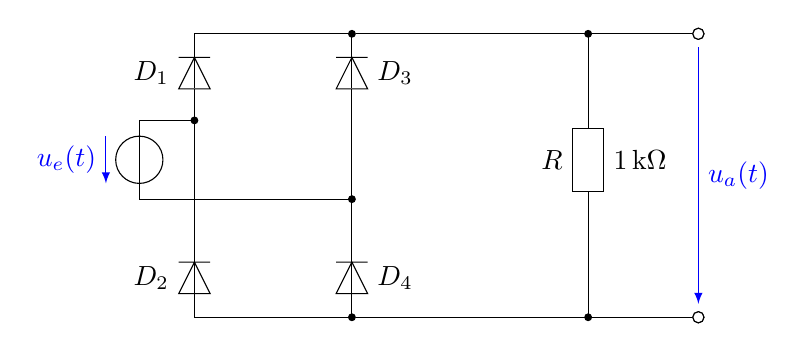
\begin{tikzpicture}
  \renewcommand{\voltagecolor}{blue}
  \voltagesourceNS{Uin}{(0.3,0)}{left}{$u_e(t)$}
  \diodeSN{diodeOne}{(1,1.3)}{left}{$D_{1}$}
  \diodeSN{diodeThree}{(3,1.3)}{right}{$D_{3}$}
  \diodeSN{diodeTwo}{(1,-1.3)}{left}{$D_{2}$}
  \diodeSN{diodeFour}{(3,-1.3)}{right}{$D_{4}$}
  \draw (UinN) -- ++(0,0.2) node (UinHelpOne) {} -- (UinHelpOne -|
      diodeOneA) \junction{UinOne};
  \draw (UinS) -- ++(0,-0.2) node (UinHelpTwo) {} -- (UinHelpTwo -|
      diodeThreeA) \junction{UinTwo};
  \draw (diodeOneA) -- (diodeTwoC) (diodeThreeA) -- (diodeFourC);

  \draw (diodeThreeC) -- ++(0,0.3) \junction{jThree} -| (diodeOneC);
  \draw (diodeFourA) -- ++(0,-0.3) \junction{jFour} -| (diodeTwoA);
  \resistorNS{resistor}{(6,0)}{$R$}{\SI{1}{\kilo\ohm}}
  \draw (jThree) -| (resistorN);
  \draw (jFour) -| (resistorS);
  \draw (jThree -| resistor) \junction{jrN} -- ++(1.4,0)
      \terminal{tuOutPlus};
  \draw (jFour -| resistor) \junction{jrS} -- (jFour -| tuOutPlus)
      \terminal{tuOutMinus};
  \voltagearrow{(tuOutPlus)}{(tuOutMinus)}{right,midway}{$u_{a}(t)$}
\end{tikzpicture}

\end{center}

\begingroup
  \fontsize{10pt}{12pt}\selectfont
  \verbatiminput{rectifier.tex}
\endgroup


\subsection{Strain Gauges Bridge}

\begin{center}
    \begin{tikzpicture}
  \renewcommand{\voltagecolor}{black}
  \opampNormInv{op}{(0,0)}
  \resistorWE{rOne}{(opInMinus)++(-2,0)}{$R_{1}=\SI{150}{\ohm}$}{}
  \resistorWE{rThree}{(opInPlus-|rOne)}{}{$R_{3} = \SI{150}{\ohm}$}
  \resistorWE{rTwo}{(op)++(0,2)}{$R_{2}$}{$\SI{1}{\mega\ohm}$}
  \draw (rOneE) -- (opInMinus) \mjunction{jopInMinus};
  \draw (rThreeE) -- (opInPlus) \mjunction{jopInPlus};
  \resistorNS{rFour}{(jopInPlus)++(0,-2)}{$R_{4}$}{$\SI{1}{\mega\ohm}$}
  \path (op) ++(-6,0) \cnode{dms};
  \foreach \x/\y/\name in {-0.8/1.2/One, -0.8/-1.2/Two, 0.8/1.2/Three,
                            0.8/-1.2/Four}{%
      \resistorNS{dms\name}{(dms)++(\x,\y)}{$ $}{$ $}
      \draw[-latex] (dms)++(\x,\y) ++(-0.4,-0.4) -- ++(0.8,0.8);
  }
  \draw (dmsOneN) -- ++(0,0.8) \cnode{foo};
  \draw (dmsThreeN) -- (dmsThree|-foo) -- (foo) \mjunction{jdmsN};
  \draw (jdmsN) -- ++(0,0.8) \terminal{tudmsPlus} node [left] {\SI{15}{\volt}};
  \draw (dmsTwoS) -- ++(0,-0.8) \cnode{foo};
  \draw (dmsFourS) -- (dmsFour|-foo) -- (foo) \mjunction{jdmsS};
  \draw (jdmsS) -- ++(0,-0.5) \cnode{gnddms};
  \gnd{(gnddms)}
  \draw (dmsOneS) -- (dmsTwoN) (rOneW) -- (rOne-|dmsOne) \junction{jLeft};
  \draw (dmsThreeS) -- (dmsFourN);
  \draw (rThreeW) -- (rThree-|dmsThree) \junction{jRight};
  \draw (jopInPlus) -- (rFourN) (rFourS) -- ++(0,-0.5) \cnode{gndRFour};
  \gnd{(gndRFour)}
  \draw (jopInMinus) |- (rTwoW);
  \draw (opOut) -- ++(1,0) \junction{jopOut} |- (rTwoE);
  \draw (jopOut) -- ++(1,0) \terminal{tuaPlus};
  \draw (tuaPlus|-gnddms) \cnode{gndOut} -- ++(0,0.5) \terminal{tuaMinus};
  \gnd{(gndOut)}
  \voltagearrow{(tuaPlus)}{(tuaMinus)}{right}{$u_{a}$}
\end{tikzpicture}

\end{center}

\begingroup
  \fontsize{10pt}{12pt}\selectfont
  \verbatiminput{bridge.tex}
\endgroup


\subsection{Astable Multivibrator}

\begin{center}
    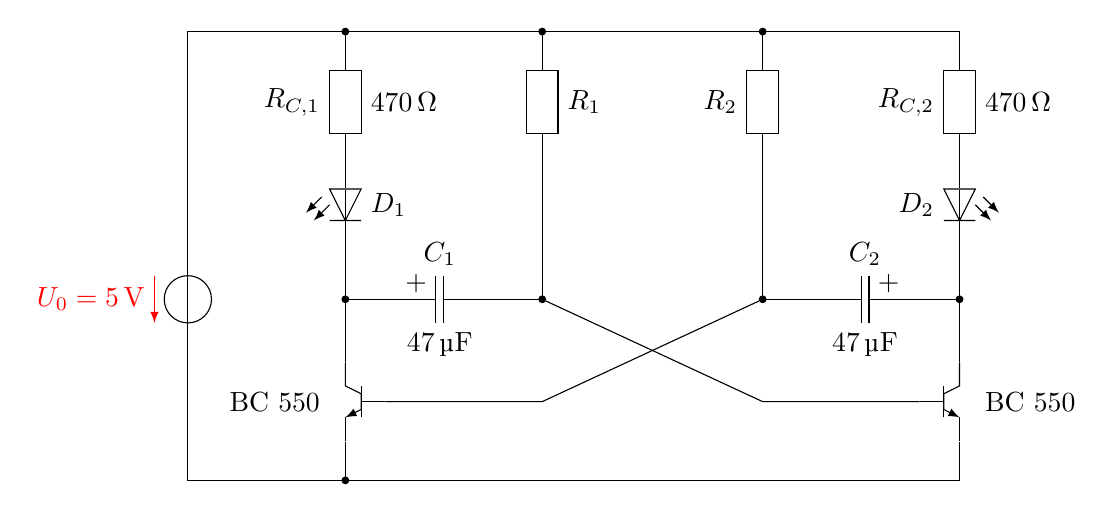
\begin{tikzpicture}
  \renewcommand{\voltagecolor}{red}
  \BJTnpnNSMirror{bjtOne}{(0,0)}
  \path (bjtOne) ++(-0.2,0) node[left] {BC 550};
  \BJTnpnNS{bjtTwo}{(bjtOne)++(7.8,0)}
  \path (bjtTwo) ++(0.2,0) node [right] {BC 550};
  \ledNSW{ledOne}{(bjtOneC)++(0,1.8)}{$D_{1}$}
  \ledNSE{ledTwo}{(bjtTwoC |- ledOne)}{$D_{2}$}
  \resistorNS{rcOne}{(ledOne)++(0,1.5)}{$R_{C,1}$}{$\SI{470}{\ohm}$}
  \resistorNS{rcTwo}{(ledTwo |- rcOne)}{$R_{C,2}$}{$\SI{470}{\ohm}$}
  \capacitorWE{cOne}{(ledOne)++(1.2,-1)}{$C_{1}$}{$\SI{47}{\micro\farad}$}
  \path (cOne)++(-0.3,0.2) node {$+$};
  \resistorNS{rOne}{(rcOne)++(2.5,0)}{}{$R_{1}$}
  \resistorNS{rTwo}{(rcTwo)++(-2.5,0)}{$R_{2}$}{}
  \capacitorWE{cTwo}{(ledTwo)++(-1.2,-1)}{$C_{2}$}{$\SI{47}{\micro\farad}$}
  \path (cTwo)++(0.3,0.2) node {$+$};
  \voltagesourceNS{u}{(ledOne |- cOne)++(-2,0)}{left}{$U_{0}=\SI{5}{\volt}$}
  \draw (rcOneN) -- ++(0,0.5) \junction{jrcN} -| (uN);
  \draw (bjtOneE) -- ++(0,-0.5) \junction{jbjtE} -| (uS);
  \draw (jrcN) -| (rcTwoN);
  \draw (jbjtE) -| (bjtTwoE);
  \draw (rOneN) -- (rOne |- jrcN) \junction{jrOneN};
  \draw (rTwoN) -- (rTwo |- jrcN) \junction{jrTwoN};
  \draw (rcOneS) -- (ledOneA) (ledOneC) -- (bjtOneC);
  \draw (rcTwoS) -- (ledTwoA) (ledTwoC) -- (bjtTwoC);
  \draw (bjtOneC |- cOne) \junction{jbjtOneC} -- (cOneW);
  \draw (bjtTwoC |- cTwo) \junction{jbjtTwoC} -- (cTwoE);
  \draw (cOneE) -- (cOne -| rOne) \junction{jcOneW} -- (rOneS);
  \draw (cTwoW) -- (cTwo -| rTwo) \junction{jcTwoE} -- (rTwoS);
  \draw (jcOneW) -- (rTwo |- bjtTwo) -- (bjtTwoB);
  \draw (jcTwoE) -- (rOne |- bjtOne) -- (bjtOneB);
\end{tikzpicture}

\end{center}

\begingroup
  \fontsize{10pt}{12pt}\selectfont
  \verbatiminput{astableMultivibrator.tex}
\endgroup


\section{Sources}

\subsection{Voltage Source in North-South Orientation}

\begin{verbatim}
\voltagesourceNS{name}{position}{align:left|right}{text}
\end{verbatim}
node endings: N: north, S: south

Example:\\
\begin{minipage}{0.8\textwidth}
\begin{verbatim}
\renewcommand{\voltagecolor}{blue}
\renewcommand{\fillcolor}{lightgray}
\voltagesourceNS{u}{(0,0)}{left}{\SI{1}{\volt}}
\draw (uN) -- ++(0,0.5) (uS) -- ++(0,-0.5);
\end{verbatim}
\end{minipage}
\begin{minipage}{0.19\textwidth}
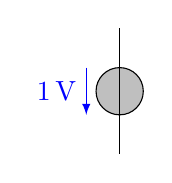
\begin{tikzpicture}
  \renewcommand{\voltagecolor}{blue}
  \renewcommand{\fillcolor}{lightgray}
  \voltagesourceNS{u}{(0,0)}{left}{\SI{1}{\volt}}
  \draw (uN) -- ++(0,0.5) (uS) -- ++(0,-0.5);

\end{tikzpicture}
\end{minipage}

\subsection{Voltage Source in South-North Orientation}

\begin{verbatim}
\voltagesourceSN{name}{position}{align:left|right}{text}
\end{verbatim}
node endings: N: north, S: south

Example:\\
\begin{minipage}{0.8\textwidth}
\begin{verbatim}
\renewcommand{\voltagecolor}{blue}
\voltagesourceSN{Ua}{(0,0)}{left}{\SI{10}{\volt}}
\draw (uN) -- ++(0,0.5) (uS) -- ++(0,-0.5);
\end{verbatim}
\end{minipage}
\begin{minipage}{0.19\textwidth}
\begin{tikzpicture}
  \renewcommand{\voltagecolor}{blue}
  \voltagesourceSN{Ua}{(0,0)}{left}{\SI{10}{\volt}}
  \draw (uN) -- ++(0,0.5) (uS) -- ++(0,-0.5);

\end{tikzpicture}
\end{minipage}

\subsection{Voltage Source in West-East Orientation}

\begin{verbatim}
\voltagesourceWE{name}{position}{align:above|below}{text}
\end{verbatim}
node endings: W: west, E: east

Example:\\
\begin{minipage}{0.8\textwidth}
\begin{verbatim}
\voltagesourceWE{u}{(0,0)}{above}{\SI{1}{\volt}}
\draw (uW) -- ++(-0.5,0) (uE) -- ++(0.5,0);
\end{verbatim}
\end{minipage}
\begin{minipage}{0.19\textwidth}
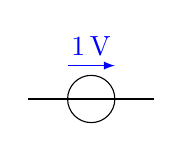
\begin{tikzpicture}
  \voltagesourceWE{u}{(0,0)}{above}{\SI{1}{\volt}}
  \draw (uW) -- ++(-0.5,0) (uE) -- ++(0.5,0);

\end{tikzpicture}
\end{minipage}

\subsection{Voltage Source in East-West Orientation}

\begin{verbatim}
\voltagesourceEW{name}{position}{align:above|below}{text}
\end{verbatim}
node endings: W: west, E: east

Example:\\
\begin{minipage}{0.8\textwidth}
\begin{verbatim}
\voltagesourceEW{u}{(0,0)}{below}{\SI{5}{\volt}}
\draw (uW) -- ++(-0.5,0) (uE) -- ++(0.5,0);
\end{verbatim}
\end{minipage}
\begin{minipage}{0.19\textwidth}
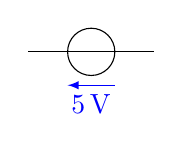
\begin{tikzpicture}
  \voltagesourceEW{u}{(0,0)}{below}{\SI{5}{\volt}}
  \draw (uW) -- ++(-0.5,0) (uE) -- ++(0.5,0);

\end{tikzpicture}
\end{minipage}

\subsection{Battery in North-South Orientation}

\begin{verbatim}
\batteryNS{name}{position}{left text}{right text}
\end{verbatim}
node endings: N: north, S: south

Example:\\
\begin{minipage}{0.8\textwidth}
\begin{verbatim}
\batteryNS{u}{(0,0)}{$U_{b}$}{\SI{1}{\volt}}
\draw (uN) -- ++(0,0.5) (uS) -- ++(0,-0.5);
\end{verbatim}
\end{minipage}
\begin{minipage}{0.19\textwidth}
\begin{tikzpicture}
  \batteryNS{u}{(0,0)}{$U_{b}$}{\SI{1}{\volt}}
  \draw (uN) -- ++(0,0.5) (uS) -- ++(0,-0.5);

\end{tikzpicture}
\end{minipage}

\subsection{Battery in South-North Orientation}

\begin{verbatim}
\batterySN{name}{position}{left text}{right text}
\end{verbatim}
node endings: N: north, S: south

Example:\\
\begin{minipage}{0.8\textwidth}
\begin{verbatim}
\batterySN{u}{(0,0)}{$U_{b}$}{\SI{1}{\volt}}
\draw (uN) -- ++(0,0.5) (uS) -- ++(0,-0.5);
\end{verbatim}
\end{minipage}
\begin{minipage}{0.19\textwidth}
\begin{tikzpicture}
  \batterySN{u}{(0,0)}{$U_{b}$}{\SI{1}{\volt}}
  \draw (uN) -- ++(0,0.5) (uS) -- ++(0,-0.5);

\end{tikzpicture}
\end{minipage}

\subsection{Current Source in North-South Orientation}

\begin{verbatim}
\currentsourceNS{name}{position}{align:left|right}{text}
\end{verbatim}
node endings: N: north, S: south

Example:\\
\begin{minipage}{0.8\textwidth}
\begin{verbatim}
\renewcommand{\currentcolor}{green}
\currentsourceNS{i}{(0,0)}{right}{$I$}
\draw (iN) -- ++(0,0.5) (iS) -- ++(0,-0.5);
\end{verbatim}
\end{minipage}
\begin{minipage}{0.19\textwidth}
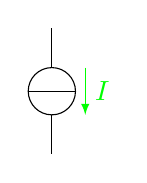
\begin{tikzpicture}
  \renewcommand{\currentcolor}{green}
  \currentsourceNS{i}{(0,0)}{right}{$I$}
  \draw (iN) -- ++(0,0.5) (iS) -- ++(0,-0.5);

\end{tikzpicture}
\end{minipage}

\subsection{Current Source in South-North Orientation}

\begin{verbatim}
\currentsourceSN{name}{position}{align:left|right}{text}
\end{verbatim}
node endings: N: north, S: south

Example:\\
\begin{minipage}{0.8\textwidth}
\begin{verbatim}
\renewcommand{\currentcolor}{red}
\currentsourceSN{i}{(0,0)}{right}{$I$}
\draw (iN) -- ++(0,0.5) (iS) -- ++(0,-0.5);
\end{verbatim}
\end{minipage}
\begin{minipage}{0.19\textwidth}
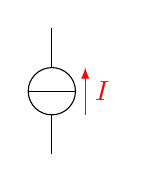
\begin{tikzpicture}
  \renewcommand{\currentcolor}{red}
  \currentsourceSN{i}{(0,0)}{right}{$I$}
  \draw (iN) -- ++(0,0.5) (iS) -- ++(0,-0.5);

\end{tikzpicture}
\end{minipage}

\subsection{Current Source in West-East Orientation}

\begin{verbatim}
\currentsourceWE{name}{position}{align:above|below}{text}
\end{verbatim}
node endings: W: west, E: east

Example:\\
\begin{minipage}{0.8\textwidth}
\begin{verbatim}
\currentsourceWE{i}{(0,0)}{above}{$I$}
\draw (iW) -- ++(-0.5,0) (iE) -- ++(0.5,0);
\end{verbatim}
\end{minipage}
\begin{minipage}{0.19\textwidth}
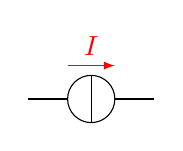
\begin{tikzpicture}
  \currentsourceWE{i}{(0,0)}{above}{$I$}
  \draw (iW) -- ++(-0.5,0) (iE) -- ++(0.5,0);

\end{tikzpicture}
\end{minipage}

\subsection{Current Source in East-West Orientation}

\begin{verbatim}
\currentsourceEW{name}{position}{align:above|below}{text}
\end{verbatim}
node endings: W: west, E: east

Example:\\
\begin{minipage}{0.8\textwidth}
\begin{verbatim}
\currentsourceEW{i}{(0,0)}{above}{$I$}
\draw (iW) -- ++(-0.5,0) (iE) -- ++(0.5,0);
\end{verbatim}
\end{minipage}
\begin{minipage}{0.19\textwidth}
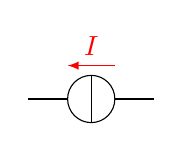
\begin{tikzpicture}
  \currentsourceEW{i}{(0,0)}{above}{$I$}
  \draw (iW) -- ++(-0.5,0) (iE) -- ++(0.5,0);

\end{tikzpicture}
\end{minipage}

\section{Voltage and Current Arrows}

\subsection{Voltage Arrow Between Two Nodes}

\begin{verbatim}
\voltagearrow{begin}{end}{text parameters}{text}
\end{verbatim}

Example:\\
\begin{minipage}{0.8\textwidth}
\begin{verbatim}
\draw (0,1) -- (1,1) \terminal{tOne};
\draw (0,0) -- (1,0) \terminal{tTwo};
\voltagearrow{(tOne)}{(tTwo)}{right}{$U$}
\end{verbatim}
\end{minipage}
\begin{minipage}{0.19\textwidth}
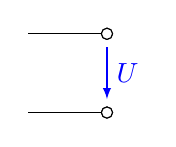
\begin{tikzpicture}
  \draw (0,1) -- (1,1) \terminal{tOne};
  \draw (0,0) -- (1,0) \terminal{tTwo};
  \voltagearrow{(tOne)}{(tTwo)}{right}{$U$}

\end{tikzpicture}
\end{minipage}

\subsection{Curved Voltage Arrow Between Two Nodes}

\begin{verbatim}
\voltagearrowC{begin}{end}{control option}{text parameters}{text}
\end{verbatim}

Example:\\
\begin{minipage}{0.8\textwidth}
\begin{verbatim}
\draw (0,1) -- (1,1) \terminal{tA};
\draw (0,0) -- (1,0) \terminal{tB};
\voltagearrowC{(tA)}{(tB)}{+(1,0) and +(1,0)}{left}{$U$}
\end{verbatim}
\end{minipage}
\begin{minipage}{0.19\textwidth}
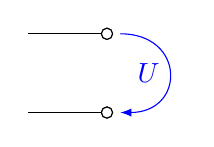
\begin{tikzpicture}
  \draw (0,1) -- (1,1) \terminal{tA};
  \draw (0,0) -- (1,0) \terminal{tB};
  \voltagearrowC{(tA)}{(tB)}{+(1,0) and +(1,0)}{left}{$U$}

\end{tikzpicture}
\end{minipage}

\subsection{Current Arrow in North-South Orientation}

\begin{verbatim}
\currentarrowNS{position}{align:left|right}{text}
\end{verbatim}

Example:\\
\begin{minipage}{0.8\textwidth}
\begin{verbatim}
\draw (0,0) -- (0,1) \mnode{ia};
\currentarrowNS{(ia)}{left}{$I$}
\end{verbatim}
\end{minipage}
\begin{minipage}{0.19\textwidth}
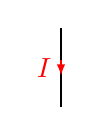
\begin{tikzpicture}
  \draw (0,0) -- (0,1) \mnode{ia};
  \currentarrowNS{(ia)}{left}{$I$}

\end{tikzpicture}
\end{minipage}

\subsection{Current Arrow in South-North Orientation}

\begin{verbatim}
\currentarrowSN{position}{align:left|right}{text}
\end{verbatim}

Example:\\
\begin{minipage}{0.8\textwidth}
\begin{verbatim}
\draw (0,0) -- (0,1) \mnode{ia};
\currentarrowSN{(ia)}{left}{$I$}
\end{verbatim}
\end{minipage}
\begin{minipage}{0.19\textwidth}
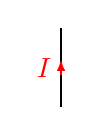
\begin{tikzpicture}
  \draw (0,0) -- (0,1) \mnode{ia};
  \currentarrowSN{(ia)}{left}{$I$}

\end{tikzpicture}
\end{minipage}

\subsection{Current Arrow in West-East Orientation}

\begin{verbatim}
\currentarrowWE{position}{align:above|below}{text}
\end{verbatim}

Example:\\
\begin{minipage}{0.8\textwidth}
\begin{verbatim}
\draw (0,0) -- (1,0) \mnode{ia};
\currentarrowWE{(ia)}{above}{$I$}
\end{verbatim}
\end{minipage}
\begin{minipage}{0.19\textwidth}
\begin{tikzpicture}
  \draw (0,0) -- (1,0) \mnode{ia};
  \currentarrowWE{(ia)}{above}{$I$}

\end{tikzpicture}
\end{minipage}

\subsection{Current Arrow in East-West Orientation}

\begin{verbatim}
\currentarrowEW{position}{align:above|below}{text}
\end{verbatim}

Example:\\
\begin{minipage}{0.8\textwidth}
\begin{verbatim}
\draw (0,0) -- (1,0) \mnode{ia};
\currentarrowEW{(ia)}{above}{$I$}
\end{verbatim}
\end{minipage}
\begin{minipage}{0.19\textwidth}
\begin{tikzpicture}
  \draw (0,0) -- (1,0) \mnode{ia};
  \currentarrowEW{(ia)}{above}{$I$}

\end{tikzpicture}
\end{minipage}

\section{Resistors, Capacitors and Inductors}

\subsection{Resistor in West-East Orientation}

\begin{verbatim}
\resistorWE{name}{position}{text above}{text below}
\end{verbatim}
node endings: W: west, E: east

Example:\\
\begin{minipage}{0.8\textwidth}
\begin{verbatim}
\resistorWE{r}{(0,0)}{$R_{1}$}{\SI{1}{\ohm}}
\draw (rW) -- ++(-0.5,0) (rE) -- ++(0.5,0);
\end{verbatim}
\end{minipage}
\begin{minipage}{0.19\textwidth}
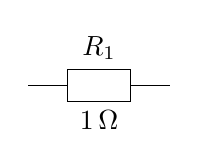
\begin{tikzpicture}
  \resistorWE{r}{(0,0)}{$R_{1}$}{\SI{1}{\ohm}}
  \draw (rW) -- ++(-0.5,0) (rE) -- ++(0.5,0);

\end{tikzpicture}
\end{minipage}

\subsection{Resistor in North-South Orientation}

\begin{verbatim}
\resistorWE{name}{position}{text left}{text right}
\end{verbatim}
node endings: N: north, S: south

Example:\\
\begin{minipage}{0.8\textwidth}
\begin{verbatim}
\resistorNS{r}{(0,0)}{$R_{1}$}{ }
\draw (rN) -- ++(0,0.5) (rS) -- ++(0,-0.5);
\end{verbatim}
\end{minipage}
\begin{minipage}{0.19\textwidth}
\begin{tikzpicture}
  \resistorNS{r}{(0,0)}{$R_{1}$}{ }
  \draw (rN) -- ++(0,0.5) (rS) -- ++(0,-0.5);

\end{tikzpicture}
\end{minipage}

\subsection{Capacitor in West-East Orientation}

\begin{verbatim}
\capacitorWE{name}{position}{text above}{text below}
\end{verbatim}
node endings: W: west, E: east

Example:\\
\begin{minipage}{0.8\textwidth}
\begin{verbatim}
\capacitorWE{c}{(0,0)}{$C_{1}$}{\SI{1}{\micro\farad}}
\draw (cW) -- ++(-0.5,0) (cE) -- ++(0.5,0);
\end{verbatim}
\end{minipage}
\begin{minipage}{0.19\textwidth}
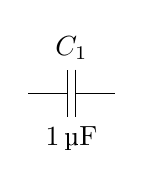
\begin{tikzpicture}
  \capacitorWE{c}{(0,0)}{$C_{1}$}{\SI{1}{\micro\farad}}
  \draw (cW) -- ++(-0.5,0) (cE) -- ++(0.5,0);

\end{tikzpicture}
\end{minipage}

\subsection{Capacitor in North-South Orientation}

\begin{verbatim}
\capacitorNS{name}{position}{text left}{text right}
\end{verbatim}
node endings: N: north, S: south

Example:\\
\begin{minipage}{0.8\textwidth}
\begin{verbatim}
\capacitorNS{c}{(0,0)}{$C_{1}$}{\SI{1}{\micro\farad}}
\draw (cN) -- ++(0,0.5) (cS) -- ++(0,-0.5);
\end{verbatim}
\end{minipage}
\begin{minipage}{0.19\textwidth}
\begin{tikzpicture}
  \capacitorNS{c}{(0,0)}{$C_{1}$}{\SI{1}{\micro\farad}}
  \draw (cN) -- ++(0,0.5) (cS) -- ++(0,-0.5);

\end{tikzpicture}
\end{minipage}

\subsection{Inductor in West-East Orientation}

\begin{verbatim}
\inductorWE{name}{position}{text above}{text below}
\end{verbatim}
node endings: W: west, E: east

Example:\\
\begin{minipage}{0.8\textwidth}
\begin{verbatim}
\inductorWE{l}{(0,0)}{$L_{1}$}{\SI{1}{\micro\henry}}
\draw (lW) -- ++(-0.5,0) (lE) -- ++(0.5,0);
\end{verbatim}
\end{minipage}
\begin{minipage}{0.19\textwidth}
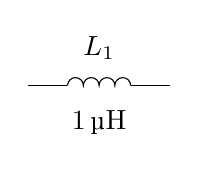
\begin{tikzpicture}
  \inductorWE{l}{(0,0)}{$L_{1}$}{\SI{1}{\micro\henry}}
  \draw (lW) -- ++(-0.5,0) (lE) -- ++(0.5,0);

\end{tikzpicture}
\end{minipage}

\subsection{Inductor in North-South Orientation}

\begin{verbatim}
\inductorNS{name}{position}{text left}{text right}
\end{verbatim}
node endings: N: north, S: south

Example:\\
\begin{minipage}{0.8\textwidth}
\begin{verbatim}
\inductorNS{l}{(0,0)}{$L_{1}$}{\SI{1}{\micro\henry}}
\draw (lN) -- ++(0,0.5) (lS) -- ++(0,-0.5);
\end{verbatim}
\end{minipage}
\begin{minipage}{0.19\textwidth}
\begin{tikzpicture}
  \inductorNS{l}{(0,0)}{$L_{1}$}{\SI{1}{\micro\henry}}
  \draw (lN) -- ++(0,0.5) (lS) -- ++(0,-0.5);

\end{tikzpicture}
\end{minipage}

\subsection{Inductor in North-South Orientation (Mirrored)}

\begin{verbatim}
\inductorNS{name}{position}{text left}{text right}
\end{verbatim}
node endings: N: north, S: south

Example:\\
\begin{minipage}{0.8\textwidth}
\begin{verbatim}
\inductorNSmirror{l}{(0,0)}{$L$}{\SI{1}{\micro\henry}}
\draw (lN) -- ++(0,0.5) (lS) -- ++(0,-0.5);
\end{verbatim}
\end{minipage}
\begin{minipage}{0.19\textwidth}
\begin{tikzpicture}
  \inductorNSmirror{l}{(0,0)}{$L$}{\SI{1}{\micro\henry}}
  \draw (lN) -- ++(0,0.5) (lS) -- ++(0,-0.5);

\end{tikzpicture}
\end{minipage}

\subsection{Varistor in West-East Orientation}

\begin{verbatim}
\varistorWE{name}{position}{text left}{text right}{controlling voltage}
\end{verbatim}
node endings: W: west, E: east

Example:\\
\begin{minipage}{0.8\textwidth}
\begin{verbatim}
\varistorWE{r}{(0,0)}{$R_{1}$}{}{$U_{v}$}
\draw (rW) -- ++(-0.5,0) (rE) -- ++(0.5,0);
\end{verbatim}
\end{minipage}
\begin{minipage}{0.19\textwidth}
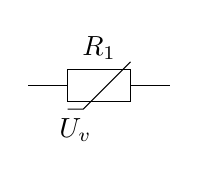
\begin{tikzpicture}
  \varistorWE{r}{(0,0)}{$R_{1}$}{}{$U_{v}$}
  \draw (rW) -- ++(-0.5,0) (rE) -- ++(0.5,0);

\end{tikzpicture}
\end{minipage}

\subsection{Potentiometer in West-East Orientation, North Connection}

\begin{verbatim}
\potentiometerWEN{name}{position}{text}
\end{verbatim}
node endings: W: west, E: east, N: north

Example:\\
\begin{minipage}{0.8\textwidth}
\begin{verbatim}
\potentiometerWEN{p}{(0,0)}{$R_{1}$}
\draw (pW) -- ++(-0.5,0) (pE) -- ++(0.5,0);
\draw (pN) |- ++(0.5,0.5);
\end{verbatim}
\end{minipage}
\begin{minipage}{0.19\textwidth}
\begin{tikzpicture}
  \potentiometerWEN{p}{(0,0)}{$R_{1}$}
  \draw (pW) -- ++(-0.5,0) (pE) -- ++(0.5,0);
  \draw (pN) |- ++(0.5,0.5);

\end{tikzpicture}
\end{minipage}

\subsection{Potentiometer in West-East Orientation, South Connection}

\begin{verbatim}
\potentiometerWES{name}{position}{text}
\end{verbatim}
node endings: W: west, E: east, S: south

Example:\\
\begin{minipage}{0.8\textwidth}
\begin{verbatim}
\potentiometerWES{p}{(0,0)}{$R_{1}$}
\draw (pW) -- ++(-0.5,0) (pE) -- ++(0.5,0);
\draw (pS) |- ++(0.5,-0.5);
\end{verbatim}
\end{minipage}
\begin{minipage}{0.19\textwidth}
\begin{tikzpicture}
  \potentiometerWES{p}{(0,0)}{$R_{1}$}
  \draw (pW) -- ++(-0.5,0) (pE) -- ++(0.5,0);
  \draw (pS) |- ++(0.5,-0.5);

\end{tikzpicture}
\end{minipage}

\subsection{Potentiometer in North-South Orientation, East Connection}

\begin{verbatim}
\potentiometerNSE{name}{position}{text}
\end{verbatim}
node endings: N: north, S: south, E: east

Example:\\
\begin{minipage}{0.8\textwidth}
\begin{verbatim}
\potentiometerNSE{p}{(0,0)}{$R_{1}$}
\draw (pS) -- ++(0,-0.5) (pN) -- ++(0,0.5);
\draw (pE) -- ++(0.5,0);
\end{verbatim}
\end{minipage}
\begin{minipage}{0.19\textwidth}
\begin{tikzpicture}
  \potentiometerNSE{p}{(0,0)}{$R_{1}$}
  \draw (pS) -- ++(0,-0.5) (pN) -- ++(0,0.5);
  \draw (pE) -- ++(0.5,0);

\end{tikzpicture}
\end{minipage}

\subsection{Potentiometer in North-South Orientation, West Connection}

\begin{verbatim}
\potentiometerNSW{name}{position}{text}
\end{verbatim}
node endings: N: north, S: south, W: west

Example:\\
\begin{minipage}{0.8\textwidth}
\begin{verbatim}
\potentiometerNSW{p}{(0,0)}{$R_{1}$}
\draw (pS) -- ++(0,-0.5) (pN) -- ++(0,0.5);
\draw (pW) -- ++(-0.5,0);
\end{verbatim}
\end{minipage}
\begin{minipage}{0.19\textwidth}
\begin{tikzpicture}
  \potentiometerNSW{p}{(0,0)}{$R_{1}$}
  \draw (pS) -- ++(0,-0.5) (pN) -- ++(0,0.5);
  \draw (pW) -- ++(-0.5,0);

\end{tikzpicture}
\end{minipage}

\section{Transformer}

\subsection{Transformer in North-South Orientation}

\begin{verbatim}
\transformerNS{name}{position}
\end{verbatim}
node endings: N: north, S: south

Example:\\
\begin{minipage}{0.8\textwidth}
\begin{verbatim}
\transformerNS{tf}{(0,0)}
\draw (tfAN) -- ++(-0.5,0) (tfAS) -- ++(-0.5,0);
\draw (tfBN) -- ++( 0.5,0) (tfBS) -- ++( 0.5,0);
\end{verbatim}
\end{minipage}
\begin{minipage}{0.19\textwidth}
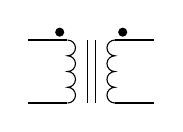
\begin{tikzpicture}
  \transformerNS{tf}{(0,0)}
  \draw (tfAN) -- ++(-0.5,0) (tfAS) -- ++(-0.5,0);
  \draw (tfBN) -- ++( 0.5,0) (tfBS) -- ++( 0.5,0);

\end{tikzpicture}
\end{minipage}

\section{Diodes}

\subsection{Diode In North-South Orientation}

\begin{verbatim}
\diodeNS{name}{position}{align:left|right}{text}
\end{verbatim}
node endings: A: anode, C: cathode

Example:\\
\begin{minipage}{0.8\textwidth}
\begin{verbatim}
\diodeNS{d}{(0,0)}{left}{$D_{1}$}
\draw (dA) -- ++(0,0.5) (dC) -- ++(0,-0.5);
\end{verbatim}
\end{minipage}
\begin{minipage}{0.19\textwidth}
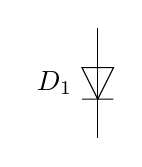
\begin{tikzpicture}
  \diodeNS{d}{(0,0)}{left}{$D_{1}$}
  \draw (dA) -- ++(0,0.5) (dC) -- ++(0,-0.5);

\end{tikzpicture}
\end{minipage}

\subsection{Diode in South-North Orientation}

\begin{verbatim}
\diodeSN{name}{position}{align:left|right}{text}
\end{verbatim}
node endings: A: anode, C: cathode

Example:\\
\begin{minipage}{0.8\textwidth}
\begin{verbatim}
\diodeSN{d}{(0,0)}{right}{$D_{1}$}
\draw (dA) -- ++(0,-0.5) (dC) -- ++(0,0.5);
\end{verbatim}
\end{minipage}
\begin{minipage}{0.19\textwidth}
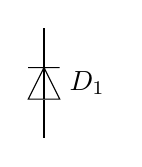
\begin{tikzpicture}
  \diodeSN{d}{(0,0)}{right}{$D_{1}$}
  \draw (dA) -- ++(0,-0.5) (dC) -- ++(0,0.5);

\end{tikzpicture}
\end{minipage}

\subsection{Diode in West-East Orientation}

\begin{verbatim}
\diodeWE{name}{position}{align:above|below}{text}
\end{verbatim}
node endings: A: anode, C: cathode

Example:\\
\begin{minipage}{0.8\textwidth}
\begin{verbatim}
\diodeWE{d}{(0,0)}{above}{$D_{1}$}
\draw (dA) -- ++(-0.5,0) (dC) -- ++(0.5,0);
\end{verbatim}
\end{minipage}
\begin{minipage}{0.19\textwidth}
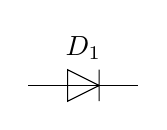
\begin{tikzpicture}
  \diodeWE{d}{(0,0)}{above}{$D_{1}$}
  \draw (dA) -- ++(-0.5,0) (dC) -- ++(0.5,0);

\end{tikzpicture}
\end{minipage}

\subsection{Diode in East-West Orientation}

\begin{verbatim}
\diodeEW{name}{position}{align:above|below}{text}
\end{verbatim}
node endings: A: anode, C: cathode

Example:\\
\begin{minipage}{0.8\textwidth}
\begin{verbatim}
\diodeEW{d}{(0,0)}{above}{$D_{1}$}
\draw (dA) -- ++(0.5,0) (dC) -- ++(-0.5,0);
\end{verbatim}
\end{minipage}
\begin{minipage}{0.19\textwidth}
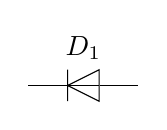
\begin{tikzpicture}
  \diodeEW{d}{(0,0)}{above}{$D_{1}$}
  \draw (dA) -- ++(0.5,0) (dC) -- ++(-0.5,0);

\end{tikzpicture}
\end{minipage}

\subsection{Zener Diode in North-South Orientation}

\begin{verbatim}
\zDiodeNS{name}{position}{align:left|right}{text}
\end{verbatim}
node endings: A: anode, C: cathode

Example:\\
\begin{minipage}{0.8\textwidth}
\begin{verbatim}
\zDiodeNS{zd}{(0,0)}{left}{$D_{1}$}
\draw (zdA) -- ++(0,0.5) (zdC) -- ++(0,-0.5);
\end{verbatim}
\end{minipage}
\begin{minipage}{0.19\textwidth}
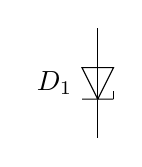
\begin{tikzpicture}
  \zDiodeNS{zd}{(0,0)}{left}{$D_{1}$}
  \draw (zdA) -- ++(0,0.5) (zdC) -- ++(0,-0.5);

\end{tikzpicture}
\end{minipage}

\subsection{Zener Diode in South-North Orientation}

\begin{verbatim}
\zDiodeSN{name}{position}{align:left|right}{text}
\end{verbatim}
node endings: A: anode, C: cathode

Example:\\
\begin{minipage}{0.8\textwidth}
\begin{verbatim}
\zDiodeSN{zd}{(0,0)}{left}{$D_{1}$}
\draw (zdA) -- ++(0,-0.5) (zdC) -- ++(0,0.5);
\end{verbatim}
\end{minipage}
\begin{minipage}{0.19\textwidth}
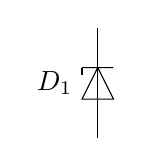
\begin{tikzpicture}
  \zDiodeSN{zd}{(0,0)}{left}{$D_{1}$}
  \draw (zdA) -- ++(0,-0.5) (zdC) -- ++(0,0.5);

\end{tikzpicture}
\end{minipage}

\subsection{Zener Diode in West-East Orientation}

\begin{verbatim}
\zDiodeWE{name}{position}{align:above|below}{text}
\end{verbatim}
node endings: A: anode, C: cathode

Example:\\
\begin{minipage}{0.8\textwidth}
\begin{verbatim}
\zDiodeWE{zd}{(0,0)}{above}{$D_{1}$}
\draw (zdA) -- ++(-0.5,0) (zdC) -- ++(0.5,0);
\end{verbatim}
\end{minipage}
\begin{minipage}{0.19\textwidth}
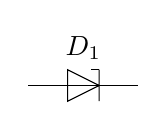
\begin{tikzpicture}
  \zDiodeWE{zd}{(0,0)}{above}{$D_{1}$}
  \draw (zdA) -- ++(-0.5,0) (zdC) -- ++(0.5,0);

\end{tikzpicture}
\end{minipage}

\subsection{Zener Diode in East-West Orientation}

\begin{verbatim}
\zDiodeEW{name}{position}{align:above|below}{text}
\end{verbatim}
node endings: A: anode, C: cathode

Example:\\
\begin{minipage}{0.8\textwidth}
\begin{verbatim}
\zDiodeEW{zd}{(0,0)}{above}{$D_{1}$}
\draw (zdA) -- ++(0.5,0) (zdC) -- ++(-0.5,0);
\end{verbatim}
\end{minipage}
\begin{minipage}{0.19\textwidth}
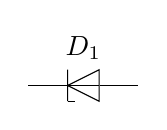
\begin{tikzpicture}
  \zDiodeEW{zd}{(0,0)}{above}{$D_{1}$}
  \draw (zdA) -- ++(0.5,0) (zdC) -- ++(-0.5,0);

\end{tikzpicture}
\end{minipage}

\subsection{LED in North-South Orientation, Light in East Direction}

\begin{verbatim}
\ledNSE{name}{position}{text}
\end{verbatim}
node endings: A: anode, C: cathode

Example:\\
\begin{minipage}{0.8\textwidth}
\begin{verbatim}
\ledNSE{led}{(0,0)}{$D_{1}$}
\draw (ledA) -- ++(0,0.5) (ledC) -- ++(0,-0.5);
\end{verbatim}
\end{minipage}
\begin{minipage}{0.19\textwidth}
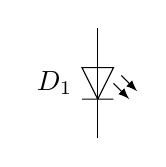
\begin{tikzpicture}
  \ledNSE{led}{(0,0)}{$D_{1}$}
  \draw (ledA) -- ++(0,0.5) (ledC) -- ++(0,-0.5);

\end{tikzpicture}
\end{minipage}

\subsection{LED in North-South Orientation, Light in West Direction}

\begin{verbatim}
\ledNSW{name}{position}{text}
\end{verbatim}
node endings: A: anode, C: cathode

Example:\\
\begin{minipage}{0.8\textwidth}
\begin{verbatim}
\ledNSW{led}{(0,0)}{$D_{1}$}
\draw (ledA) -- ++(0,0.5) (ledC) -- ++(0,-0.5);
\end{verbatim}
\end{minipage}
\begin{minipage}{0.19\textwidth}
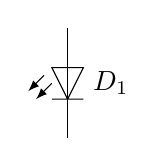
\begin{tikzpicture}
  \ledNSW{led}{(0,0)}{$D_{1}$}
  \draw (ledA) -- ++(0,0.5) (ledC) -- ++(0,-0.5);

\end{tikzpicture}
\end{minipage}

\subsection{LED in South-North Orientation, Light in West Direction}

\begin{verbatim}
\ledSNW{name}{position}{text}
\end{verbatim}
node endings: A: anode, C: cathode

Example:\\
\begin{minipage}{0.8\textwidth}
\begin{verbatim}
\ledSNW{led}{(0,0)}{$D_{1}$}
\draw (ledA) -- ++(0,-0.5) (ledC) -- ++(0,0.5);
\end{verbatim}
\end{minipage}
\begin{minipage}{0.19\textwidth}
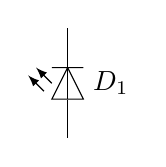
\begin{tikzpicture}
  \ledSNW{led}{(0,0)}{$D_{1}$}
  \draw (ledA) -- ++(0,-0.5) (ledC) -- ++(0,0.5);

\end{tikzpicture}
\end{minipage}

\subsection{LED in West-East orientation, Light in North Direction}

\begin{verbatim}
\ledWEN{name}{position}{text}
\end{verbatim}
node endings: A: anode, C: cathode

Example:\\
\begin{minipage}{0.8\textwidth}
\begin{verbatim}
\ledWEN{led}{(0,0)}{$D_{1}$}
\draw (ledA) -- ++(-0.5,0) (ledC) -- ++(0.5,0);
\end{verbatim}
\end{minipage}
\begin{minipage}{0.19\textwidth}
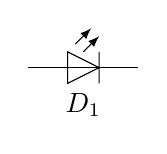
\begin{tikzpicture}
  \ledWEN{led}{(0,0)}{$D_{1}$}
  \draw (ledA) -- ++(-0.5,0) (ledC) -- ++(0.5,0);

\end{tikzpicture}
\end{minipage}

\subsection{Photo Diode in North-South Orientation, Light from East}

\begin{verbatim}
\photodiodeNSE{name}{position}{text}
\end{verbatim}
node endings: A: anode, C: cathode

Example:\\
\begin{minipage}{0.8\textwidth}
\begin{verbatim}
\photodiodeNSE{pd}{(0,0)}{$D_{1}$}
\draw (pdA) -- ++(0,0.5) (pdC) -- ++(0,-0.5);
\end{verbatim}
\end{minipage}
\begin{minipage}{0.19\textwidth}
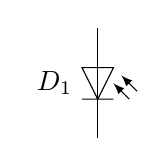
\begin{tikzpicture}
  \photodiodeNSE{pd}{(0,0)}{$D_{1}$}
  \draw (pdA) -- ++(0,0.5) (pdC) -- ++(0,-0.5);

\end{tikzpicture}
\end{minipage}

\subsection{photo diode in North-South Orientation, Light from West}

\begin{verbatim}
\photodiodeNSW{name}{position}{text}
\end{verbatim}
node endings: A: anode, C: cathode

Example:\\
\begin{minipage}{0.8\textwidth}
\begin{verbatim}
\photodiodeNSW{pd}{(0,0)}{$D_{1}$}
\draw (pdA) -- ++(0,0.5) (pdC) -- ++(0,-0.5);
\end{verbatim}
\end{minipage}
\begin{minipage}{0.19\textwidth}
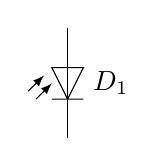
\begin{tikzpicture}
  \photodiodeNSW{pd}{(0,0)}{$D_{1}$}
  \draw (pdA) -- ++(0,0.5) (pdC) -- ++(0,-0.5);

\end{tikzpicture}
\end{minipage}

\section{Transistors}

\subsection{N-Channel JFET in North-South Orientation}

\begin{verbatim}
\nChnJFETNS{name}{position}
\end{verbatim}
node endings: D: drain, G: gate, S: source

Example:\\
\begin{minipage}{0.8\textwidth}
\begin{verbatim}
\nChnJFETNS{jfet}{(0,0)}
\path (jfetG) node [left]{G};
\path (jfetD) node [above]{D};
\path (jfetS) node [below]{S};
\end{verbatim}
\end{minipage}
\begin{minipage}{0.19\textwidth}
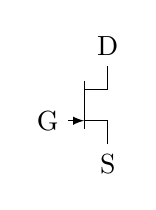
\begin{tikzpicture}
  \nChnJFETNS{jfet}{(0,0)}
  \path (jfetG) node [left]{G};
  \path (jfetD) node [above]{D};
  \path (jfetS) node [below]{S};

\end{tikzpicture}
\end{minipage}

\subsection{N-Channel JFET in West-East Orientation}

\begin{verbatim}
\nChnJFETWE{name}{position}
\end{verbatim}
node endings: D: drain, G: gate, S: source

Example:\\
\begin{minipage}{0.8\textwidth}
\begin{verbatim}
\nChnJFETWE{jfet}{(0,0)}
\path (jfetG) node [below]{G};
\path (jfetD) node [left]{D};
\path (jfetS) node [right]{S};
\end{verbatim}
\end{minipage}
\begin{minipage}{0.19\textwidth}
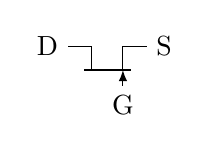
\begin{tikzpicture}
  \nChnJFETWE{jfet}{(0,0)}
  \path (jfetG) node [below]{G};
  \path (jfetD) node [left]{D};
  \path (jfetS) node [right]{S};

\end{tikzpicture}
\end{minipage}

\subsection{Enhancement-Mode N-Channel MOSFET in North-South Orientation}

\begin{verbatim}
\NMOSFETenhNS{name}{position}
\end{verbatim}
node endings: D: drain, G: gate, S: source, B: bulk

Example:\\
\begin{minipage}{0.8\textwidth}
\begin{verbatim}
\NMOSFETenhNS{jfet}{(0,0)}
\path (jfetG) node [left]{G};
\path (jfetD) node [above]{D};
\path (jfetS) node [below]{S};
\end{verbatim}
\end{minipage}
\begin{minipage}{0.19\textwidth}
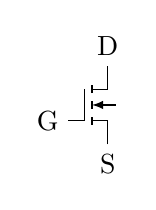
\begin{tikzpicture}
  \NMOSFETenhNS{jfet}{(0,0)}
  \path (jfetG) node [left]{G};
  \path (jfetD) node [above]{D};
  \path (jfetS) node [below]{S};

\end{tikzpicture}
\end{minipage}

\subsection{Enhancement-Mode P-Channel MOSFET in North-South Orientation}

\begin{verbatim}
\PMOSFETenhNS{name}{position}
\end{verbatim}
node endings: D: drain, G: gate, S: source, B: bulk

Example:\\
\begin{minipage}{0.8\textwidth}
\begin{verbatim}
\PMOSFETenhNS{jfet}{(0,0)}
\path (jfetG) node [left]{G};
\path (jfetD) node [above]{D};
\path (jfetS) node [below]{S};
\end{verbatim}
\end{minipage}
\begin{minipage}{0.19\textwidth}
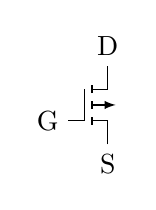
\begin{tikzpicture}
  \PMOSFETenhNS{jfet}{(0,0)}
  \path (jfetG) node [left]{G};
  \path (jfetD) node [above]{D};
  \path (jfetS) node [below]{S};

\end{tikzpicture}
\end{minipage}

\subsection{NPN Bipolar Junction Transistor in North-South Orientation}

\begin{verbatim}
\BJTnpnNS{name}{position}
\end{verbatim}
node endings: B: basis, E: emitter, C: collector

Example:\\
\begin{minipage}{0.8\textwidth}
\begin{verbatim}
\BJTnpnNS{b}{(0,0)}
\path (bB) node [left]{B};
\path (bC) node [above]{C};
\path (bE) node [below]{E};
\end{verbatim}
\end{minipage}
\begin{minipage}{0.19\textwidth}
\begin{tikzpicture}
  \BJTnpnNS{b}{(0,0)}
  \path (bB) node [left]{B};
  \path (bC) node [above]{C};
  \path (bE) node [below]{E};

\end{tikzpicture}
\end{minipage}

\subsection{NPN Bipolar Junction Transistor in North-South Orientation (Mirrored)}

\begin{verbatim}
\BJTnpnNSMirror{name}{position}
\end{verbatim}
node endings: B: basis, E: emitter, C: collector

Example:\\
\begin{minipage}{0.8\textwidth}
\begin{verbatim}
\BJTnpnNSMirror{b}{(0,0)}
\path (bB) node [right]{B};
\path (bC) node [above]{C};
\path (bE) node [below]{E};
\end{verbatim}
\end{minipage}
\begin{minipage}{0.19\textwidth}
\begin{tikzpicture}
  \BJTnpnNSMirror{b}{(0,0)}
  \path (bB) node [right]{B};
  \path (bC) node [above]{C};
  \path (bE) node [below]{E};

\end{tikzpicture}
\end{minipage}

\subsection{NPN Bipolar Junction Transistor in South-North Orientation}

\begin{verbatim}
\BJTnpnSN{name}{position}
\end{verbatim}
node endings: B: basis, E: emitter, C: collector

Example:\\
\begin{minipage}{0.8\textwidth}
\begin{verbatim}
\BJTnpnSN{b}{(0,0)}
\path (bB) node [left]{B};
\path (bC) node [below]{C};
\path (bE) node [above]{E};
\end{verbatim}
\end{minipage}
\begin{minipage}{0.19\textwidth}
\begin{tikzpicture}
  \BJTnpnSN{b}{(0,0)}
  \path (bB) node [left]{B};
  \path (bC) node [below]{C};
  \path (bE) node [above]{E};

\end{tikzpicture}
\end{minipage}

\subsection{NPN Bipolar Junction Transistor in East-West Orientation}

\begin{verbatim}
\BJTnpnEW{name}{position}
\end{verbatim}
node endings: B: basis, E: emitter, C: collector

Example:\\
\begin{minipage}{0.8\textwidth}
\begin{verbatim}
\BJTnpnEW{b}{(0,0)}
\path (bB) node [below]{B};
\path (bC) node [right]{C};
\path (bE) node [left]{E};
\end{verbatim}
\end{minipage}
\begin{minipage}{0.19\textwidth}
\begin{tikzpicture}
  \BJTnpnEW{b}{(0,0)}
  \path (bB) node [below]{B};
  \path (bC) node [right]{C};
  \path (bE) node [left]{E};

\end{tikzpicture}
\end{minipage}

\subsection{PNP Bipolar Junction Transistor in North-South Orientation}

\begin{verbatim}
\BJTpnpNS{name}{position}
\end{verbatim}
node endings: B: basis, E: emitter, C: collector

Example:\\
\begin{minipage}{0.8\textwidth}
\begin{verbatim}
\BJTpnpNS{b}{(0,0)}
\path (bB) node [left]{B};
\path (bC) node [above]{C};
\path (bE) node [below]{E};
\end{verbatim}
\end{minipage}
\begin{minipage}{0.19\textwidth}
\begin{tikzpicture}
  \BJTpnpNS{b}{(0,0)}
  \path (bB) node [left]{B};
  \path (bC) node [above]{C};
  \path (bE) node [below]{E};

\end{tikzpicture}
\end{minipage}

\section{Operational Amplifiers}

\subsection{OP-AMP, Standardized Symbol}

\begin{verbatim}
\opampNorm{name}{position}
\end{verbatim}
node endings: Out: output, InMinus: n-input, InPlus: p-input,
              UbattPlus: positive power supply,
              UbattMinus: negative power supply
              Gnd: ground

Example:\\
\begin{minipage}{0.8\textwidth}
\begin{verbatim}
\opampNorm{op}{(0,0)}
\draw (opOut) -- ++(0.5,0);
\draw (opInMinus) -- ++(-0.5,0);
\draw (opInPlus) -- ++(-0.5,0);
\draw (opUbattPlus) -- ++(0,0.3) node [above]{$+U_{0}$};
\draw (opUbattMinus) -- ++(0,-0.3) node [below]{$-U_{0}$};
\draw (opGnd) -- ++(0,-0.2) -| ++(0.3,-0.1) \cnode{gnd};
\gnd{(gnd)}
\end{verbatim}
\end{minipage}
\begin{minipage}{0.19\textwidth}
\begin{tikzpicture}
  \opampNorm{op}{(0,0)}
  \draw (opOut) -- ++(0.5,0);
  \draw (opInMinus) -- ++(-0.5,0);
  \draw (opInPlus) -- ++(-0.5,0);
  \draw (opUbattPlus) -- ++(0,0.3) node [above]{$+U_{0}$};
  \draw (opUbattMinus) -- ++(0,-0.3) node [below]{$-U_{0}$};
  \draw (opGnd) -- ++(0,-0.2) -| ++(0.3,-0.1) \cnode{gnd};
  \gnd{(gnd)}

\end{tikzpicture}
\end{minipage}

\subsection{OP-AMP, Standardized Symbol, N-Input above P-Input}

\begin{verbatim}
\opampNormInv{name}{position}
\end{verbatim}
node endings: Out: output, InMinus: n-input, InPlus: p-input,
              UbattPlus: positive power supply,
              UbattMinus: negative power supply
              Gnd: ground

Example:\\
\begin{minipage}{0.8\textwidth}
\begin{verbatim}
\opampNormInv{op}{(0,0)}
\draw (opOut) -- ++(0.5,0);
\draw (opInMinus) -- ++(-0.5,0);
\draw (opInPlus) -- ++(-0.5,0);
\draw (opUbattPlus) -- ++(0,0.3) node [above]{$+U_{0}$};
\draw (opUbattMinus) -- ++(0,-0.3) node [below]{$-U_{0}$};
\draw (opGnd) -- ++(0,-0.2) -| ++(0.3,-0.1) \cnode{gnd};
\gnd{(gnd)}
\end{verbatim}
\end{minipage}
\begin{minipage}{0.19\textwidth}
\begin{tikzpicture}
  \opampNormInv{op}{(0,0)}
  \draw (opOut) -- ++(0.5,0);
  \draw (opInMinus) -- ++(-0.5,0);
  \draw (opInPlus) -- ++(-0.5,0);
  \draw (opUbattPlus) -- ++(0,0.3) node [above]{$+U_{0}$};
  \draw (opUbattMinus) -- ++(0,-0.3) node [below]{$-U_{0}$};
  \draw (opGnd) -- ++(0,-0.2) -| ++(0.3,-0.1) \cnode{gnd};
  \gnd{(gnd)}

\end{tikzpicture}
\end{minipage}

\subsection{OP-AMP}

\begin{verbatim}
\opamp{name}{position}
\end{verbatim}
node endings: Out: output, InMinus: n-input, InPlus: p-input,
              UbattPlus: positive power supply,
              UbattMinus: negative power supply
              Gnd: ground

Example:\\
\begin{minipage}{0.8\textwidth}
\begin{verbatim}
\opamp{op}{(0,0)}
\draw (opOut) -- ++(0.5,0);
\draw (opInMinus) -- ++(-0.5,0);
\draw (opInPlus) -- ++(-0.5,0);
\draw (opUbattPlus) -- ++(0,0.3) node [above]{$+U_{0}$};
\draw (opUbattMinus) -- ++(0,-0.3) node [below]{$-U_{0}$};
\draw (opGnd) -- ++(0,-0.2) -| ++(0.3,-0.1) \cnode{gnd};
\gnd{(gnd)}
\end{verbatim}
\end{minipage}
\begin{minipage}{0.19\textwidth}
\begin{tikzpicture}
  \opamp{op}{(0,0)}
  \draw (opOut) -- ++(0.5,0);
  \draw (opInMinus) -- ++(-0.5,0);
  \draw (opInPlus) -- ++(-0.5,0);
  \draw (opUbattPlus) -- ++(0,0.3) node [above]{$+U_{0}$};
  \draw (opUbattMinus) -- ++(0,-0.3) node [below]{$-U_{0}$};
  \draw (opGnd) -- ++(0,-0.2) -| ++(0.3,-0.1) \cnode{gnd};
  \gnd{(gnd)}

\end{tikzpicture}
\end{minipage}

\subsection{OP-AMP, N-Input above P-Input}

\begin{verbatim}
\opampInv{name}{position}
\end{verbatim}
node endings: Out: output, InMinus: n-input, InPlus: p-input,
              UbattPlus: positive power supply,
              UbattMinus: negative power supply
              Gnd: ground

Example:\\
\begin{minipage}{0.8\textwidth}
\begin{verbatim}
\opampInv{opamp}{(0,0)}
\draw (opampOut) -- ++(0.5,0);
\draw (opInMinus) -- ++(-0.5,0);
\draw (opInPlus) -- ++(-0.5,0);
\draw (opUbattPlus) -- ++(0,0.3) node [above]{$+U_{0}$};
\draw (opUbattMinus) -- ++(0,-0.3) node [below]{$-U_{0}$};
\draw (opGnd) -- ++(0,-0.2) -| ++(0.3,-0.1) \cnode{gnd};
\gnd{(gnd)}
\end{verbatim}
\end{minipage}
\begin{minipage}{0.19\textwidth}
\begin{tikzpicture}
  \opampInv{opamp}{(0,0)}
  \draw (opampOut) -- ++(0.5,0);
  \draw (opInMinus) -- ++(-0.5,0);
  \draw (opInPlus) -- ++(-0.5,0);
  \draw (opUbattPlus) -- ++(0,0.3) node [above]{$+U_{0}$};
  \draw (opUbattMinus) -- ++(0,-0.3) node [below]{$-U_{0}$};
  \draw (opGnd) -- ++(0,-0.2) -| ++(0.3,-0.1) \cnode{gnd};
  \gnd{(gnd)}

\end{tikzpicture}
\end{minipage}

\subsection{General Amplifier}

\begin{verbatim}
\amplifier{name}{position}
\end{verbatim}
node endings: OutPlus: p-output OutMinus: n-output,
              InMinus: n-input, InPlus: p-input,
              UbattPlus: positive power supply,
              UbattMinus: negative power supply
              Gnd: ground

Example:\\
\begin{minipage}{0.8\textwidth}
\begin{verbatim}
\amplifier{a}{(0,0)}
\draw (aOutPlus) -- ++(0.5,0);
\draw (aOutMinus) -- ++(0.5,0);
\draw (aInMinus) -- ++(-0.5,0);
\draw (aInPlus) -- ++(-0.5,0);
\draw (aUBattPlus) -- ++(0,0.3) node [above]{$+U_{0}$};
\draw (aUBattMinus) -- ++(0,-0.3) node [below]{$-U_{0}$};
\draw (aGnd) -- ++(0,-0.2) -| ++(0.3,-0.1) \cnode{gnd};
\gnd{(gnd)}
\end{verbatim}
\end{minipage}
\begin{minipage}{0.19\textwidth}
\begin{tikzpicture}
  \amplifier{a}{(0,0)}
  \draw (aOutPlus) -- ++(0.5,0);
  \draw (aOutMinus) -- ++(0.5,0);
  \draw (aInMinus) -- ++(-0.5,0);
  \draw (aInPlus) -- ++(-0.5,0);
  \draw (aUBattPlus) -- ++(0,0.3) node [above]{$+U_{0}$};
  \draw (aUBattMinus) -- ++(0,-0.3) node [below]{$-U_{0}$};
  \draw (aGnd) -- ++(0,-0.2) -| ++(0.3,-0.1) \cnode{gnd};
  \gnd{(gnd)}

\end{tikzpicture}
\end{minipage}

\section{Amplifiers}

\subsection{Amplifier, Standardized Symbol}

\begin{verbatim}
\ampNorm{name}{position}{amplification factor}
\end{verbatim}
node endings: Out: output, InMinus: n-input, InPlus: p-input,
              UbattPlus: positive power supply,
              UbattMinus: negative power supply
              Gnd: ground

Example:\\
\begin{minipage}{0.8\textwidth}
\begin{verbatim}
\ampNorm{amp}{(0,0)}{$k$}
\draw (ampOut) -- ++(0.5,0);
\draw (ampInMinus) -- ++(-0.5,0);
\draw (ampInPlus) -- ++(-0.5,0);
\draw (ampUbattPlus) -- ++(0,0.3) node [above]{$+U_{0}$};
\draw (ampUbattMinus) -- ++(0,-0.3) node [below]{$-U_{0}$};
\draw (ampGnd) -- ++(0,-0.2) -| ++(0.3,-0.1) \cnode{gnd};
\gnd{(gnd)}
\end{verbatim}
\end{minipage}
\begin{minipage}{0.19\textwidth}
\begin{tikzpicture}
  \ampNorm{amp}{(0,0)}{$k$}
  \draw (ampOut) -- ++(0.5,0);
  \draw (ampInMinus) -- ++(-0.5,0);
  \draw (ampInPlus) -- ++(-0.5,0);
  \draw (ampUbattPlus) -- ++(0,0.3) node [above]{$+U_{0}$};
  \draw (ampUbattMinus) -- ++(0,-0.3) node [below]{$-U_{0}$};
  \draw (ampGnd) -- ++(0,-0.2) -| ++(0.3,-0.1) \cnode{gnd};
  \gnd{(gnd)}

\end{tikzpicture}
\end{minipage}

\section{Logic Gates}

\subsection{Inversion Symbol for Logic Gates Outputs}

\begin{verbatim}
\NOTcircle{name}{position}
\end{verbatim}

Example:\\
\begin{minipage}{0.8\textwidth}
\begin{verbatim}
\draw (0,0) -- (0,1);
\NOTcircle{n}{(0,0.5)}
\end{verbatim}
\end{minipage}
\begin{minipage}{0.19\textwidth}
\begin{tikzpicture}
  \draw (0,0) -- (0,1);
  \NOTcircle{n}{(0,0.5)}

\end{tikzpicture}
\end{minipage}

\subsection{Logic Gate Symbol, IEC Standard}

\begin{verbatim}
\LogicGateIEC{name}{position}
\end{verbatim}
node endings: In: input, Out: output,
              InN: north input, InS: south input,
              N: north, S: south

Example:\\
\begin{minipage}{0.8\textwidth}
\begin{verbatim}
\LogicGateIEC{g}{(0,0)}
\draw (gIn) -- ++(-0.2,0);
\draw (gOut) -- ++(0.5,0);
\draw (gInN) -- ++(-0.5,0);
\draw (gInS) -- ++(-0.5,0);
\draw (gN) -- ++(0,0.2);
\draw (gS) -- ++(0,-0.2);
\end{verbatim}
\end{minipage}
\begin{minipage}{0.19\textwidth}
\begin{tikzpicture}
  \LogicGateIEC{g}{(0,0)}
  \draw (gIn) -- ++(-0.2,0);
  \draw (gOut) -- ++(0.5,0);
  \draw (gInN) -- ++(-0.5,0);
  \draw (gInS) -- ++(-0.5,0);
  \draw (gN) -- ++(0,0.2);
  \draw (gS) -- ++(0,-0.2);

\end{tikzpicture}
\end{minipage}

\subsection{Logic AND Gate Symbol}

\begin{verbatim}
\GateAND{name}{position}
\end{verbatim}
node endings: In: input, Out: output,
              InN: north input, InS: south input,
              N: north, S: south

Example:\\
\begin{minipage}{0.8\textwidth}
\begin{verbatim}
\GateAND{g}{(0,0)}
\draw (gOut) -- ++(0.5,0);
\draw (gInN) -- ++(-0.5,0);
\draw (gInS) -- ++(-0.5,0);
\end{verbatim}
\end{minipage}
\begin{minipage}{0.19\textwidth}
\begin{tikzpicture}
  \GateAND{g}{(0,0)}
  \draw (gOut) -- ++(0.5,0);
  \draw (gInN) -- ++(-0.5,0);
  \draw (gInS) -- ++(-0.5,0);

\end{tikzpicture}
\end{minipage}

\subsection{Logic NAND Gate Symbol}

\begin{verbatim}
\GateNAND{name}{position}
\end{verbatim}
node endings: In: input, Out: output,
              InN: north input, InS: south input,
              N: north, S: south

Example:\\
\begin{minipage}{0.8\textwidth}
\begin{verbatim}
\GateNAND{g}{(0,0)}
\draw (gOut) -- ++(0.5,0);
\draw (gInN) -- ++(-0.5,0);
\draw (gInS) -- ++(-0.5,0);
\end{verbatim}
\end{minipage}
\begin{minipage}{0.19\textwidth}
\begin{tikzpicture}
  \GateNAND{g}{(0,0)}
  \draw (gOut) -- ++(0.5,0);
  \draw (gInN) -- ++(-0.5,0);
  \draw (gInS) -- ++(-0.5,0);

\end{tikzpicture}
\end{minipage}

\subsection{Logic OR Gate Symbol}

\begin{verbatim}
\GateOR{name}{position}
\end{verbatim}
node endings: In: input, Out: output,
              InN: north input, InS: south input,
              N: north, S: south

Example:\\
\begin{minipage}{0.8\textwidth}
\begin{verbatim}
\GateOR{g}{(0,0)}
\draw (gOut) -- ++(0.5,0);
\draw (gInN) -- ++(-0.5,0);
\draw (gInS) -- ++(-0.5,0);
\end{verbatim}
\end{minipage}
\begin{minipage}{0.19\textwidth}
\begin{tikzpicture}
  \GateOR{g}{(0,0)}
  \draw (gOut) -- ++(0.5,0);
  \draw (gInN) -- ++(-0.5,0);
  \draw (gInS) -- ++(-0.5,0);

\end{tikzpicture}
\end{minipage}

\subsection{Logic NOR Gate Symbol}

\begin{verbatim}
\GateNOR{name}{position}
\end{verbatim}
node endings: In: input, Out: output,
              InN: north input, InS: south input,
              N: north, S: south

Example:\\
\begin{minipage}{0.8\textwidth}
\begin{verbatim}
\GateNOR{g}{(0,0)}
\draw (gOut) -- ++(0.5,0);
\draw (gInN) -- ++(-0.5,0);
\draw (gInS) -- ++(-0.5,0);
\end{verbatim}
\end{minipage}
\begin{minipage}{0.19\textwidth}
\begin{tikzpicture}
  \GateNOR{g}{(0,0)}
  \draw (gOut) -- ++(0.5,0);
  \draw (gInN) -- ++(-0.5,0);
  \draw (gInS) -- ++(-0.5,0);

\end{tikzpicture}
\end{minipage}

\subsection{Logic NOT Gate Symbol}

\begin{verbatim}
\GateNOT{name}{position}
\end{verbatim}
node endings: In: input, Out: output,
              InN: north input, InS: south input,
              N: north, S: south

Example:\\
\begin{minipage}{0.8\textwidth}
\begin{verbatim}
\GateNOT{g}{(0,0)}
\draw (gOut) -- ++(0.5,0);
\draw (gIn) -- ++(-0.5,0);
\end{verbatim}
\end{minipage}
\begin{minipage}{0.19\textwidth}
\begin{tikzpicture}
  \GateNOT{g}{(0,0)}
  \draw (gOut) -- ++(0.5,0);
  \draw (gIn) -- ++(-0.5,0);

\end{tikzpicture}
\end{minipage}

\subsection{Logic XOR Gate Symbol}

\begin{verbatim}
\GateXOR{name}{position}
\end{verbatim}
node endings: In: input, Out: output,
              InN: north input, InS: south input,
              N: north, S: south

Example:\\
\begin{minipage}{0.8\textwidth}
\begin{verbatim}
\GateXOR{g}{(0,0)}
\draw (gOut) -- ++(0.5,0);
\draw (gInN) -- ++(-0.5,0);
\draw (gInS) -- ++(-0.5,0);
\end{verbatim}
\end{minipage}
\begin{minipage}{0.19\textwidth}
\begin{tikzpicture}
  \GateXOR{g}{(0,0)}
  \draw (gOut) -- ++(0.5,0);
  \draw (gInN) -- ++(-0.5,0);
  \draw (gInS) -- ++(-0.5,0);

\end{tikzpicture}
\end{minipage}

\subsection{Logic XNOR Gate Symbol}

\begin{verbatim}
\GateXNOR{name}{position}
\end{verbatim}
node endings: In: input, Out: output,
              InN: north input, InS: south input,
              N: north, S: south

Example:\\
\begin{minipage}{0.8\textwidth}
\begin{verbatim}
\GateXNOR{g}{(0,0)}
\draw (gOut) -- ++(0.5,0);
\draw (gInN) -- ++(-0.5,0);
\draw (gInS) -- ++(-0.5,0);
\end{verbatim}
\end{minipage}
\begin{minipage}{0.19\textwidth}
\begin{tikzpicture}
  \GateXNOR{g}{(0,0)}
  \draw (gOut) -- ++(0.5,0);
  \draw (gInN) -- ++(-0.5,0);
  \draw (gInS) -- ++(-0.5,0);

\end{tikzpicture}
\end{minipage}

\subsection{Logic AND Gate, ANSI Symbol}

\begin{verbatim}
\ANSIGateAND{name}{position}
\end{verbatim}
node endings: Out: output,
              InN: north input, InS: south input,
              N: north, S: south

Example:\\
\begin{minipage}{0.8\textwidth}
\begin{verbatim}
\ANSIGateAND{g}{(0,0)}
\draw (gOut) -- ++(0.5,0);
\draw (gInN) -- ++(-0.5,0);
\draw (gInS) -- ++(-0.5,0);
\end{verbatim}
\end{minipage}
\begin{minipage}{0.19\textwidth}
\begin{tikzpicture}
  \ANSIGateAND{g}{(0,0)}
  \draw (gOut) -- ++(0.5,0);
  \draw (gInN) -- ++(-0.5,0);
  \draw (gInS) -- ++(-0.5,0);

\end{tikzpicture}
\end{minipage}

\subsection{Logic NAND Gate, ANSI Symbol}

\begin{verbatim}
\ANSIGateNAND{name}{position}
\end{verbatim}
node endings: Out: output,
              InN: north input, InS: south input,
              N: north, S: south

Example:\\
\begin{minipage}{0.8\textwidth}
\begin{verbatim}
\ANSIGateNAND{g}{(0,0)}
\draw (gOut) -- ++(0.5,0);
\draw (gInN) -- ++(-0.5,0);
\draw (gInS) -- ++(-0.5,0);
\end{verbatim}
\end{minipage}
\begin{minipage}{0.19\textwidth}
\begin{tikzpicture}
  \ANSIGateNAND{g}{(0,0)}
  \draw (gOut) -- ++(0.5,0);
  \draw (gInN) -- ++(-0.5,0);
  \draw (gInS) -- ++(-0.5,0);

\end{tikzpicture}
\end{minipage}

\subsection{Logic OR Gate, ANSI Symbol}

\begin{verbatim}
\ANSIGateOR{name}{position}
\end{verbatim}
node endings: Out: output,
              InN: north input, InS: south input,
              N: north, S: south

Example:\\
\begin{minipage}{0.8\textwidth}
\begin{verbatim}
\ANSIGateOR{g}{(0,0)}
\draw (gOut) -- ++(0.5,0);
\draw (gInN) -- ++(-0.5,0);
\draw (gInS) -- ++(-0.5,0);
\end{verbatim}
\end{minipage}
\begin{minipage}{0.19\textwidth}
\begin{tikzpicture}
  \ANSIGateOR{g}{(0,0)}
  \draw (gOut) -- ++(0.5,0);
  \draw (gInN) -- ++(-0.5,0);
  \draw (gInS) -- ++(-0.5,0);

\end{tikzpicture}
\end{minipage}

\subsection{Logic NOR Gate, ANSI Symbol}

\begin{verbatim}
\ANSIGateNOR{name}{position}
\end{verbatim}
node endings: Out: output,
              InN: north input, InS: south input,
              N: north, S: south

Example:\\
\begin{minipage}{0.8\textwidth}
\begin{verbatim}
\ANSIGateNOR{g}{(0,0)}
\draw (gOut) -- ++(0.5,0);
\draw (gInN) -- ++(-0.5,0);
\draw (gInS) -- ++(-0.5,0);
\end{verbatim}
\end{minipage}
\begin{minipage}{0.19\textwidth}
\begin{tikzpicture}
  \ANSIGateNOR{g}{(0,0)}
  \draw (gOut) -- ++(0.5,0);
  \draw (gInN) -- ++(-0.5,0);
  \draw (gInS) -- ++(-0.5,0);

\end{tikzpicture}
\end{minipage}

\subsection{Logic NOT Gate, ANSI Symbol}

\begin{verbatim}
\ANSIGateNOT{name}{position}
\end{verbatim}
node endings: Out: output, In: input,
              N: north, S: south

Example:\\
\begin{minipage}{0.8\textwidth}
\begin{verbatim}
\ANSIGateNOT{g}{(0,0)}
\draw (gOut) -- ++(0.5,0);
\draw (gIn) -- ++(-0.5,0);
\end{verbatim}
\end{minipage}
\begin{minipage}{0.19\textwidth}
\begin{tikzpicture}
  \ANSIGateNOT{g}{(0,0)}
  \draw (gOut) -- ++(0.5,0);
  \draw (gIn) -- ++(-0.5,0);

\end{tikzpicture}
\end{minipage}

\subsection{Logic XOR Gate, ANSI Symbol}

\begin{verbatim}
\ANSIGateXOR{name}{position}
\end{verbatim}
node endings: Out: output,
              InN: north input, InS: south input,
              N: north, S: south

Example:\\
\begin{minipage}{0.8\textwidth}
\begin{verbatim}
\ANSIGateXOR{g}{(0,0)}
\draw (gOut) -- ++(0.5,0);
\draw (gInN) -- ++(-0.5,0);
\draw (gInS) -- ++(-0.5,0);
\end{verbatim}
\end{minipage}
\begin{minipage}{0.19\textwidth}
\begin{tikzpicture}
  \ANSIGateXOR{g}{(0,0)}
  \draw (gOut) -- ++(0.5,0);
  \draw (gInN) -- ++(-0.5,0);
  \draw (gInS) -- ++(-0.5,0);

\end{tikzpicture}
\end{minipage}

\subsection{Logic XNOR Gate, ANSI Symbol}

\begin{verbatim}
\ANSIGateXNOR{name}{position}
\end{verbatim}
node endings: Out: output,
              InN: north input, InS: south input,
              N: north, S: south

Example:\\
\begin{minipage}{0.8\textwidth}
\begin{verbatim}
\ANSIGateXNOR{g}{(0,0)}
\draw (gOut) -- ++(0.5,0);
\draw (gInN) -- ++(-0.5,0);
\draw (gInS) -- ++(-0.5,0);
\end{verbatim}
\end{minipage}
\begin{minipage}{0.19\textwidth}
\begin{tikzpicture}
  \ANSIGateXNOR{g}{(0,0)}
  \draw (gOut) -- ++(0.5,0);
  \draw (gInN) -- ++(-0.5,0);
  \draw (gInS) -- ++(-0.5,0);

\end{tikzpicture}
\end{minipage}

\section{Flip-Flops}

\subsection{General Flip-Flop Symbol}

\begin{verbatim}
\FlipFlop{name}{position}
\end{verbatim}
node endings: OutN: north output, OutS: south output
              InN: north input, InS: south input,
              N: north, S: south
              W: middle input

Example:\\
\begin{minipage}{0.8\textwidth}
\begin{verbatim}
\FlipFlop{ff}{(0,0)}
\draw (ffInN) -- ++(-0.5,0) (ffInS) -- ++(-0.5,0);
\draw (ffOutN) -- ++(0.5,0) (ffOutS) -- ++(0.5,0);
\end{verbatim}
\end{minipage}
\begin{minipage}{0.19\textwidth}
\begin{tikzpicture}
  \FlipFlop{ff}{(0,0)}
  \draw (ffInN) -- ++(-0.5,0) (ffInS) -- ++(-0.5,0);
  \draw (ffOutN) -- ++(0.5,0) (ffOutS) -- ++(0.5,0);

\end{tikzpicture}
\end{minipage}

\subsection{General Flip-Flop Symbol for Negative Logic}

\begin{verbatim}
\FlipFlopNegLogic{name}{position}
\end{verbatim}
node endings: OutN: north output, OutS: south output
              InN: north input, InS: south input,
              N: north, S: south
              W: middle input

Example:\\
\begin{minipage}{0.8\textwidth}
\begin{verbatim}
\FlipFlopNegLogic{ff}{(0,0)}
\draw (ffInN) -- ++(-0.5,0) (ffInS) -- ++(-0.5,0);
\draw (ffOutN) -- ++(0.5,0) (ffOutS) -- ++(0.5,0);
\end{verbatim}
\end{minipage}
\begin{minipage}{0.19\textwidth}
\begin{tikzpicture}
  \FlipFlopNegLogic{ff}{(0,0)}
  \draw (ffInN) -- ++(-0.5,0) (ffInS) -- ++(-0.5,0);
  \draw (ffOutN) -- ++(0.5,0) (ffOutS) -- ++(0.5,0);

\end{tikzpicture}
\end{minipage}

\subsection{Flip-Flop Changing on Rising Edge}

\begin{verbatim}
\FlipFlopRisingEdge{name}{position}
\end{verbatim}
node endings: OutN: north output, OutS: south output
              InN: north input, InS: south input,
              N: north, S: south
              W: middle input

Example:\\
\begin{minipage}{0.8\textwidth}
\begin{verbatim}
\FlipFlopRisingEdge{ff}{(0,0)}
\draw (ffInN) -- ++(-0.5,0) (ffInS) -- ++(-0.5,0);
\draw (ffW) -- ++(-0.5,0);
\draw (ffOutN) -- ++(0.5,0) (ffOutS) -- ++(0.5,0);
\end{verbatim}
\end{minipage}
\begin{minipage}{0.19\textwidth}
\begin{tikzpicture}
  \FlipFlopRisingEdge{ff}{(0,0)}
  \draw (ffInN) -- ++(-0.5,0) (ffInS) -- ++(-0.5,0);
  \draw (ffW) -- ++(-0.5,0);
  \draw (ffOutN) -- ++(0.5,0) (ffOutS) -- ++(0.5,0);

\end{tikzpicture}
\end{minipage}

\subsection{Flip-Flop Changing on Falling Edge}

\begin{verbatim}
\FlipFlopFallingEdge{name}{position}
\end{verbatim}
node endings: OutN: north output, OutS: south output
              InN: north input, InS: south input,
              N: north, S: south
              W: middle input

Example:\\
\begin{minipage}{0.8\textwidth}
\begin{verbatim}
\FlipFlopFallingEdge{ff}{(0,0)}
\draw (ffInN) -- ++(-0.5,0) (ffInS) -- ++(-0.5,0);
\draw (ffInC) -- ++(-0.5,0);
\draw (ffOutN) -- ++(0.5,0) (ffOutS) -- ++(0.5,0);
\end{verbatim}
\end{minipage}
\begin{minipage}{0.19\textwidth}
\begin{tikzpicture}
  \FlipFlopFallingEdge{ff}{(0,0)}
  \draw (ffInN) -- ++(-0.5,0) (ffInS) -- ++(-0.5,0);
  \draw (ffInC) -- ++(-0.5,0);
  \draw (ffOutN) -- ++(0.5,0) (ffOutS) -- ++(0.5,0);

\end{tikzpicture}
\end{minipage}

\subsection{RS Flip-Flop}

\begin{verbatim}
\RSFlipFlop{name}{position}
\end{verbatim}
node endings: OutN: north output, OutS: south output
              InN: north input, InS: south input,
              N: north, S: south
              W: middle input

Example:\\
\begin{minipage}{0.8\textwidth}
\begin{verbatim}
\RSFlipFlop{ff}{(0,0)}
\draw (ffInN) -- ++(-0.5,0) (ffInS) -- ++(-0.5,0);
\draw (ffOutN) -- ++(0.5,0) (ffOutS) -- ++(0.5,0);
\end{verbatim}
\end{minipage}
\begin{minipage}{0.19\textwidth}
\begin{tikzpicture}
  \RSFlipFlop{ff}{(0,0)}
  \draw (ffInN) -- ++(-0.5,0) (ffInS) -- ++(-0.5,0);
  \draw (ffOutN) -- ++(0.5,0) (ffOutS) -- ++(0.5,0);

\end{tikzpicture}
\end{minipage}

\subsection{RS NAND Flip-Flop (Negative Logic)}

\begin{verbatim}
\RSNANDFlipFlop{name}{position}
\end{verbatim}
node endings: OutN: north output, OutS: south output
              InN: north input, InS: south input,
              N: north, S: south
              W: middle input

Example:\\
\begin{minipage}{0.8\textwidth}
\begin{verbatim}
\RSNANDFlipFlop{ff}{(0,0)}
\draw (ffInN) -- ++(-0.5,0) (ffInS) -- ++(-0.5,0);
\draw (ffOutN) -- ++(0.5,0) (ffOutS) -- ++(0.5,0);
\end{verbatim}
\end{minipage}
\begin{minipage}{0.19\textwidth}
\begin{tikzpicture}
  \RSNANDFlipFlop{ff}{(0,0)}
  \draw (ffInN) -- ++(-0.5,0) (ffInS) -- ++(-0.5,0);
  \draw (ffOutN) -- ++(0.5,0) (ffOutS) -- ++(0.5,0);

\end{tikzpicture}
\end{minipage}

\subsection{RS Flip-Flop Changing on Rising Edge}

\begin{verbatim}
\RSFlipFlopRisingEdge{name}{position}
\end{verbatim}
node endings: OutN: north output, OutS: south output
              InN: north input, InS: south input,
              N: north, S: south
              W: middle input

Example:\\
\begin{minipage}{0.8\textwidth}
\begin{verbatim}
\RSFlipFlopRisingEdge{ff}{(0,0)}
\draw (ffInN) -- ++(-0.5,0) (ffInS) -- ++(-0.5,0);
\draw (ffW) -- ++(-0.5,0);
\draw (ffOutN) -- ++(0.5,0) (ffOutS) -- ++(0.5,0);
\end{verbatim}
\end{minipage}
\begin{minipage}{0.19\textwidth}
\begin{tikzpicture}
  \RSFlipFlopRisingEdge{ff}{(0,0)}
  \draw (ffInN) -- ++(-0.5,0) (ffInS) -- ++(-0.5,0);
  \draw (ffW) -- ++(-0.5,0);
  \draw (ffOutN) -- ++(0.5,0) (ffOutS) -- ++(0.5,0);

\end{tikzpicture}
\end{minipage}

\subsection{RS Flip-Flop Changing on Falling Edge}

\begin{verbatim}
\RSFlipFlopFallingEdge{name}{position}
\end{verbatim}
node endings: OutN: north output, OutS: south output
              InN: north input, InS: south input,
              N: north, S: south
              W: middle input

Example:\\
\begin{minipage}{0.8\textwidth}
\begin{verbatim}
\RSFlipFlopFallingEdge{ff}{(0,0)}
\draw (ffInN) -- ++(-0.5,0) (ffInS) -- ++(-0.5,0);
\draw (ffInC) -- ++(-0.5,0);
\draw (ffOutN) -- ++(0.5,0) (ffOutS) -- ++(0.5,0);
\end{verbatim}
\end{minipage}
\begin{minipage}{0.19\textwidth}
\begin{tikzpicture}
  \RSFlipFlopFallingEdge{ff}{(0,0)}
  \draw (ffInN) -- ++(-0.5,0) (ffInS) -- ++(-0.5,0);
  \draw (ffInC) -- ++(-0.5,0);
  \draw (ffOutN) -- ++(0.5,0) (ffOutS) -- ++(0.5,0);

\end{tikzpicture}
\end{minipage}

\subsection{JK Flip-Flop Changing on Rising Edge}

\begin{verbatim}
\JKFlipFlopRisingEdge{name}{position}
\end{verbatim}
node endings: OutN: north output, OutS: south output
              InN: north input, InS: south input,
              N: north, S: south
              W: middle input

Example:\\
\begin{minipage}{0.8\textwidth}
\begin{verbatim}
\JKFlipFlopRisingEdge{ff}{(0,0)}
\draw (ffInN) -- ++(-0.5,0) (ffInS) -- ++(-0.5,0);
\draw (ffW) -- ++(-0.5,0);
\draw (ffOutN) -- ++(0.5,0) (ffOutS) -- ++(0.5,0);
\end{verbatim}
\end{minipage}
\begin{minipage}{0.19\textwidth}
\begin{tikzpicture}
  \JKFlipFlopRisingEdge{ff}{(0,0)}
  \draw (ffInN) -- ++(-0.5,0) (ffInS) -- ++(-0.5,0);
  \draw (ffW) -- ++(-0.5,0);
  \draw (ffOutN) -- ++(0.5,0) (ffOutS) -- ++(0.5,0);

\end{tikzpicture}
\end{minipage}

\subsection{JK Master-Slave Flip-Flop}

\begin{verbatim}
\JKMSFlipFlop{name}{position}
\end{verbatim}
node endings: OutN: north output, OutS: south output
              InN: north input, InS: south input,
              N: north, S: south
              W: middle input

Example:\\
\begin{minipage}{0.8\textwidth}
\begin{verbatim}
\JKMSFlipFlop{ff}{(0,0)}
\draw (ffInN) -- ++(-0.5,0) (ffInS) -- ++(-0.5,0);
\draw (ffW) -- ++(-0.5,0);
\draw (ffOutN) -- ++(0.5,0) (ffOutS) -- ++(0.5,0);
\end{verbatim}
\end{minipage}
\begin{minipage}{0.19\textwidth}
\begin{tikzpicture}
  \JKMSFlipFlop{ff}{(0,0)}
  \draw (ffInN) -- ++(-0.5,0) (ffInS) -- ++(-0.5,0);
  \draw (ffW) -- ++(-0.5,0);
  \draw (ffOutN) -- ++(0.5,0) (ffOutS) -- ++(0.5,0);

\end{tikzpicture}
\end{minipage}

\subsection{D Flip-Flop Changing on Rising Edge}

\begin{verbatim}
\DFlipFlopRisingEdge{name}{position}
\end{verbatim}
node endings: OutN: north output, OutS: south output
              InN: north input, InS: south input,
              N: north, S: south
              W: middle input

Example:\\
\begin{minipage}{0.8\textwidth}
\begin{verbatim}
\DFlipFlopRisingEdge{ff}{(0,0)}
\draw (ffInN) -- ++(-0.5,0);
\draw (ffW) -- ++(-0.5,0);
\draw (ffOutN) -- ++(0.5,0) (ffOutS) -- ++(0.5,0);
\end{verbatim}
\end{minipage}
\begin{minipage}{0.19\textwidth}
\begin{tikzpicture}
  \DFlipFlopRisingEdge{ff}{(0,0)}
  \draw (ffInN) -- ++(-0.5,0);
  \draw (ffW) -- ++(-0.5,0);
  \draw (ffOutN) -- ++(0.5,0) (ffOutS) -- ++(0.5,0);

\end{tikzpicture}
\end{minipage}

\subsection{T Flip-Flop Changing on Rising Edge}

\begin{verbatim}
\TFlipFlopRisingEdge{name}{position}
\end{verbatim}
node endings: OutN: north output, OutS: south output
              InN: north input, InS: south input,
              N: north, S: south
              W: middle input

Example:\\
\begin{minipage}{0.8\textwidth}
\begin{verbatim}
\TFlipFlopRisingEdge{ff}{(0,0)}
\draw (ffW) -- ++(-0.5,0);
\draw (ffOutN) -- ++(0.5,0) (ffOutS) -- ++(0.5,0);
\end{verbatim}
\end{minipage}
\begin{minipage}{0.19\textwidth}
\begin{tikzpicture}
  \TFlipFlopRisingEdge{ff}{(0,0)}
  \draw (ffW) -- ++(-0.5,0);
  \draw (ffOutN) -- ++(0.5,0) (ffOutS) -- ++(0.5,0);

\end{tikzpicture}
\end{minipage}

\subsection{T Flip-Flop Changing on Falling Edge}

\begin{verbatim}
\TFlipFlopFallingEdge{name}{position}
\end{verbatim}
node endings: OutN: north output, OutS: south output
              InN: north input, InS: south input,
              N: north, S: south
              W: middle input

Example:\\
\begin{minipage}{0.8\textwidth}
\begin{verbatim}
\TFlipFlopFallingEdge{ff}{(0,0)}
\draw (ffInC) -- ++(-0.5,0);
\draw (ffOutN) -- ++(0.5,0) (ffOutS) -- ++(0.5,0);
\end{verbatim}
\end{minipage}
\begin{minipage}{0.19\textwidth}
\begin{tikzpicture}
  \TFlipFlopFallingEdge{ff}{(0,0)}
  \draw (ffInC) -- ++(-0.5,0);
  \draw (ffOutN) -- ++(0.5,0) (ffOutS) -- ++(0.5,0);

\end{tikzpicture}
\end{minipage}

\subsection{Monoflop}

\begin{verbatim}
\Monoflop{name}{position}
\end{verbatim}
node endings: OutN: north output, OutS: south output
              InN: north input, InS: south input,
              N: north, S: south
              W: middle input

Example:\\
\begin{minipage}{0.8\textwidth}
\begin{verbatim}
\Monoflop{ff}{(0,0)}
\draw (ffInN) -- ++(-0.5,0) (ffInS) -- ++(-0.5,0);
\draw (ffOutN) -- ++(0.5,0) (ffOutS) -- ++(0.5,0);
\end{verbatim}
\end{minipage}
\begin{minipage}{0.19\textwidth}
\begin{tikzpicture}
  \Monoflop{ff}{(0,0)}
  \draw (ffInN) -- ++(-0.5,0) (ffInS) -- ++(-0.5,0);
  \draw (ffOutN) -- ++(0.5,0) (ffOutS) -- ++(0.5,0);

\end{tikzpicture}
\end{minipage}

\subsection{Switch, West-East Direction}

\begin{verbatim}
\switchWE{name}{position}
\end{verbatim}
node endings: W: west, E: east, N: north connection

Example:\\
\begin{minipage}{0.8\textwidth}
\begin{verbatim}
\switchWE{s}{(0,0)}
\draw (sW) -- ++(-0.5,0) (sE) -- ++(0.5,0);
\end{verbatim}
\end{minipage}
\begin{minipage}{0.19\textwidth}
\begin{tikzpicture}
  \switchWE{s}{(0,0)}
  \draw (sW) -- ++(-0.5,0) (sE) -- ++(0.5,0);

\end{tikzpicture}
\end{minipage}

\subsection{Closed Switch, West-East Direction}

\begin{verbatim}
\switchClosedWE{name}{position}
\end{verbatim}
node endings: W: west, E: east, N: north connection

Example:\\
\begin{minipage}{0.8\textwidth}
\begin{verbatim}
\switchClosedWE{s}{(0,0)}
\draw (sW) -- ++(-0.5,0) (sE) -- ++(0.5,0);
\end{verbatim}
\end{minipage}
\begin{minipage}{0.19\textwidth}
\begin{tikzpicture}
  \switchClosedWE{s}{(0,0)}
  \draw (sW) -- ++(-0.5,0) (sE) -- ++(0.5,0);

\end{tikzpicture}
\end{minipage}

\subsection{Switch, East-West Direction}

\begin{verbatim}
\switchEW{name}{position}
\end{verbatim}
node endings: W: west, E: east, N: north connection

Example:\\
\begin{minipage}{0.8\textwidth}
\begin{verbatim}
\switchEW{s}{(0,0)}
\draw (sW) -- ++(-0.5,0) (sE) -- ++(0.5,0);
\end{verbatim}
\end{minipage}
\begin{minipage}{0.19\textwidth}
\begin{tikzpicture}
  \switchEW{s}{(0,0)}
  \draw (sW) -- ++(-0.5,0) (sE) -- ++(0.5,0);

\end{tikzpicture}
\end{minipage}

\subsection{Closed Switch, East-West Direction}

\begin{verbatim}
\switchClosedEW{name}{position}
\end{verbatim}
node endings: W: west, E: east, N: north connection

Example:\\
\begin{minipage}{0.8\textwidth}
\begin{verbatim}
\switchClosedEW{s}{(0,0)}
\draw (sW) -- ++(-0.5,0) (sE) -- ++(0.5,0);
\end{verbatim}
\end{minipage}
\begin{minipage}{0.19\textwidth}
\begin{tikzpicture}
  \switchClosedEW{s}{(0,0)}
  \draw (sW) -- ++(-0.5,0) (sE) -- ++(0.5,0);

\end{tikzpicture}
\end{minipage}

\subsection{Switch, South-North Direction}

\begin{verbatim}
\switchSN{name}{position}
\end{verbatim}
node endings: S: south, N: north, W: west connection

Example:\\
\begin{minipage}{0.8\textwidth}
\begin{verbatim}
\switchSN{s}{(0,0)}
\draw (sS) -- ++(0,-0.5) (sN) -- ++(0,0.5);
\end{verbatim}
\end{minipage}
\begin{minipage}{0.19\textwidth}
\begin{tikzpicture}
  \switchSN{s}{(0,0)}
  \draw (sS) -- ++(0,-0.5) (sN) -- ++(0,0.5);

\end{tikzpicture}
\end{minipage}

\subsection{Closed Switch, South-North Direction}

\begin{verbatim}
\switchClosedSN{name}{position}
\end{verbatim}
node endings: S: south, N: north, W: west connection

Example:\\
\begin{minipage}{0.8\textwidth}
\begin{verbatim}
\switchClosedSN{s}{(0,0)}
\draw (sS) -- ++(0,-0.5) (sN) -- ++(0,0.5);
\end{verbatim}
\end{minipage}
\begin{minipage}{0.19\textwidth}
\begin{tikzpicture}
  \switchClosedSN{s}{(0,0)}
  \draw (sS) -- ++(0,-0.5) (sN) -- ++(0,0.5);

\end{tikzpicture}
\end{minipage}

\subsection{Pushbutton, West-East Direction}

\begin{verbatim}
\pushbuttonWE{name}{position}
\end{verbatim}
node endings: W: west, E: east, N: north connection

Example:\\
\begin{minipage}{0.8\textwidth}
\begin{verbatim}
\pushbuttonWE{b}{(0,0)}
\draw (bW) -- ++(-0.5,0) (bE) -- ++(0.5,0);
\end{verbatim}
\end{minipage}
\begin{minipage}{0.19\textwidth}
\begin{tikzpicture}
  \pushbuttonWE{b}{(0,0)}
  \draw (bW) -- ++(-0.5,0) (bE) -- ++(0.5,0);

\end{tikzpicture}
\end{minipage}

\subsection{Pushbutton, South-North Direction}

\begin{verbatim}
\pushbuttonSN{name}{position}
\end{verbatim}
node endings: S: south, N: north, W: west connection

Example:\\
\begin{minipage}{0.8\textwidth}
\begin{verbatim}
\pushbuttonSN{b}{(0,0)}
\draw (bS) -- ++(0,-0.5) (bN) -- ++(0,0.5);
\end{verbatim}
\end{minipage}
\begin{minipage}{0.19\textwidth}
\begin{tikzpicture}
  \pushbuttonSN{b}{(0,0)}
  \draw (bS) -- ++(0,-0.5) (bN) -- ++(0,0.5);

\end{tikzpicture}
\end{minipage}

\section{Miscellaneous}

\subsection{Ground as Symbol}

\begin{verbatim}
\gnd{position}
\end{verbatim}

Example:\\
\begin{minipage}{0.8\textwidth}
\begin{verbatim}
\draw (0,0) -- (1,0) \junction{gnd};
\gnd{(gnd)}
\end{verbatim}
\end{minipage}
\begin{minipage}{0.19\textwidth}
\begin{tikzpicture}
  \draw (0,0) -- (1,0) \junction{gnd};
  \gnd{(gnd)}

\end{tikzpicture}
\end{minipage}

\subsection{Ground as Continued Drawing}

\begin{verbatim}
\gndNow
\end{verbatim}

Example:\\
\begin{minipage}{0.8\textwidth}
\begin{verbatim}
\draw (0,0) -- (1,0) \junction{foo} \gndNow;
\end{verbatim}
\end{minipage}
\begin{minipage}{0.19\textwidth}
\begin{tikzpicture}
  \draw (0,0) -- (1,0) \junction{foo} \gndNow;

\end{tikzpicture}
\end{minipage}

\subsection{Connecting Terminal}

\begin{verbatim}
\terminal{name}
\end{verbatim}
node endings: Con: use terminal as connector (no space when wired)

Example:\\
\begin{minipage}{0.8\textwidth}
\begin{verbatim}
\renewcommand{\fillcolor}{white}
\draw (0,0) -- ++(1,0) \terminal{t};
\end{verbatim}
\end{minipage}
\begin{minipage}{0.19\textwidth}
\begin{tikzpicture}
  \renewcommand{\fillcolor}{white}
  \draw (0,0) -- ++(1,0) \terminal{t};

\end{tikzpicture}
\end{minipage}

\subsection{Junction (Black Filled Circle)}

\begin{verbatim}
\junction{name}
\end{verbatim}

Example:\\
\begin{minipage}{0.8\textwidth}
\begin{verbatim}
\draw (0,0) -- (1,0);
\draw (0.5,0) \junction{j} -- ++(0,-0.5);
\end{verbatim}
\end{minipage}
\begin{minipage}{0.19\textwidth}
\begin{tikzpicture}
  \draw (0,0) -- (1,0);
  \draw (0.5,0) \junction{j} -- ++(0,-0.5);

\end{tikzpicture}
\end{minipage}

\subsection{Junction in the Middle of a Path}

\begin{verbatim}
\junction{name}
\end{verbatim}

Example:\\
\begin{minipage}{0.8\textwidth}
\begin{verbatim}
\draw (0,0) -- (1,0) \mjunction{j} (j) -- ++(1,0);
\end{verbatim}
\end{minipage}
\begin{minipage}{0.19\textwidth}
\begin{tikzpicture}
  \draw (0,0) -- (1,0) \mjunction{j} (j) -- ++(1,0);

\end{tikzpicture}
\end{minipage}

\subsection{Connection Node (for Referencing, not Visible)}

\begin{verbatim}
\cnode{name}
\end{verbatim}

Example:\\
\begin{minipage}{0.8\textwidth}
\begin{verbatim}
\draw (0,0) -- (0.5,0) \cnode{c} -- (0.5,0.5);
\draw (c) -- ++(0,-0.5);
\end{verbatim}
\end{minipage}
\begin{minipage}{0.19\textwidth}
\begin{tikzpicture}
  \draw (0,0) -- (0.5,0) \cnode{c} -- (0.5,0.5);
  \draw (c) -- ++(0,-0.5);

\end{tikzpicture}
\end{minipage}

\subsection{Midway Connection Node}

\begin{verbatim}
\mnode{name}
\end{verbatim}

Example:\\
\begin{minipage}{0.8\textwidth}
\begin{verbatim}
\draw (0,0) -- (1,0) \mnode{m};
\draw (m) -- ++(0,-0.5);
\end{verbatim}
\end{minipage}
\begin{minipage}{0.19\textwidth}
\begin{tikzpicture}
  \draw (0,0) -- (1,0) \mnode{m};
  \draw (m) -- ++(0,-0.5);

\end{tikzpicture}
\end{minipage}

\subsection{Invisible Node with Terminal Node Properties (Used with Voltage Arrows)}

\begin{verbatim}
\node{name}
\end{verbatim}

Example:\\
\begin{minipage}{0.8\textwidth}
\begin{verbatim}
\draw (0,0) -- ++(1,0) \tnode{t};
\end{verbatim}
\end{minipage}
\begin{minipage}{0.19\textwidth}
\begin{tikzpicture}
  \draw (0,0) -- ++(1,0) \tnode{t};

\end{tikzpicture}
\end{minipage}

\subsection{Speaker}

\begin{verbatim}
\speakerWE{name}{position}
\end{verbatim}
node endings: N: north, S: south,

Example:\\
\begin{minipage}{0.8\textwidth}
\begin{verbatim}
\speakerWE{sp}{(0,0)}
\draw (spN) -- ++(0,0.5) (spS) -- ++(0,-0.5);
\end{verbatim}
\end{minipage}
\begin{minipage}{0.19\textwidth}
\begin{tikzpicture}
  \speakerWE{sp}{(0,0)}
  \draw (spN) -- ++(0,0.5) (spS) -- ++(0,-0.5);

\end{tikzpicture}
\end{minipage}

\subsection{Bulb}

\begin{verbatim}
\bulb{name}{position}
\end{verbatim}
node endings: N: north, S: south, W: west, E: east

Example:\\
\begin{minipage}{0.8\textwidth}
\begin{verbatim}
\bulb{b}{(0,0)}
\draw (bN) -- ++(0,0.5) (bS) -- ++(0,-0.5);
\end{verbatim}
\end{minipage}
\begin{minipage}{0.19\textwidth}
\begin{tikzpicture}
  \bulb{b}{(0,0)}
  \draw (bN) -- ++(0,0.5) (bS) -- ++(0,-0.5);

\end{tikzpicture}
\end{minipage}

\subsection{Multimeter (Circle for Voltmeter or Ammeter)}

\begin{verbatim}
\multimeter{name}{position}{letter}
\end{verbatim}
node endings: N: north, S: south, W: west, E: east

Example:\\
\begin{minipage}{0.8\textwidth}
\begin{verbatim}
\multimeter{m}{(0,0)}{M}
\draw (mN) -- ++(0,0.5) (mS) -- ++(0,-0.5);
\end{verbatim}
\end{minipage}
\begin{minipage}{0.19\textwidth}
\begin{tikzpicture}
  \multimeter{m}{(0,0)}{M}
  \draw (mN) -- ++(0,0.5) (mS) -- ++(0,-0.5);

\end{tikzpicture}
\end{minipage}

\subsection{Voltmeter}

\begin{verbatim}
\voltmeter{name}{position}
\end{verbatim}
node endings: N: north, S: south, W: west, E: east

Example:\\
\begin{minipage}{0.8\textwidth}
\begin{verbatim}
\voltmeter{v}{(0,0)}
\draw (vN) -- ++(0,0.5) (vS) -- ++(0,-0.5);
\end{verbatim}
\end{minipage}
\begin{minipage}{0.19\textwidth}
\begin{tikzpicture}
  \voltmeter{v}{(0,0)}
  \draw (vN) -- ++(0,0.5) (vS) -- ++(0,-0.5);

\end{tikzpicture}
\end{minipage}

\subsection{Ammeter}

\begin{verbatim}
\ammeter{name}{position}
\end{verbatim}
node endings: N: north, S: south, W: west, E: east

Example:\\
\begin{minipage}{0.8\textwidth}
\begin{verbatim}
\ammeter{a}{(0,0)}
\draw (vW) -- ++(-0.5,0) (vE) -- ++(0.5,0);
\end{verbatim}
\end{minipage}
\begin{minipage}{0.19\textwidth}
\begin{tikzpicture}
  \ammeter{a}{(0,0)}
  \draw (vW) -- ++(-0.5,0) (vE) -- ++(0.5,0);

\end{tikzpicture}
\end{minipage}

\subsection{Brushless DC Electric Motor}

\begin{verbatim}
\BLDCMotor{name}{position}{pin1}{pin2}
\end{verbatim}
node endings: N: north, S: south, W: west, E: east

Example:\\
\begin{minipage}{0.8\textwidth}
\begin{verbatim}
\BLDCMotor{motor}{(0,0)}{$A_1$}{$A_2$}
\draw (motorN) -- ++(0,0.5);
\draw (motorS) -- ++(0,-0.5);
\end{verbatim}
\end{minipage}
\begin{minipage}{0.19\textwidth}
\begin{tikzpicture}
  \BLDCMotor{motor}{(0,0)}{$A_1$}{$A_2$}
  \draw (motorN) -- ++(0,0.5);
  \draw (motorS) -- ++(0,-0.5);

\end{tikzpicture}
\end{minipage}

\subsection{Brushless DC Electric Generator}

\begin{verbatim}
\BLDCGenerator{name}{position}{pin1}{pin2}
\end{verbatim}
node endings: N: north, S: south, W: west, E: east

Example:\\
\begin{minipage}{0.8\textwidth}
\begin{verbatim}
\BLDCGenerator{gen}{(0,0)}{$A_1$}{$A_2$}
\draw (genN) -- ++(0,0.5);
\draw (genS) -- ++(0,-0.5);
\end{verbatim}
\end{minipage}
\begin{minipage}{0.19\textwidth}
\begin{tikzpicture}
  \BLDCGenerator{gen}{(0,0)}{$A_1$}{$A_2$}
  \draw (genN) -- ++(0,0.5);
  \draw (genS) -- ++(0,-0.5);

\end{tikzpicture}
\end{minipage}

\subsection{Brushes for Electric Motors and Generators}

\begin{verbatim}
\brushes{position}
\end{verbatim}
Only usful in combination with motors or generators.

Example:\\
\begin{minipage}{0.8\textwidth}
\begin{verbatim}
\brushes{(0,0)}
\end{verbatim}
\end{minipage}
\begin{minipage}{0.19\textwidth}
\begin{tikzpicture}
  \brushes{(0,0)}

\end{tikzpicture}
\end{minipage}

\subsection{Brushless DC Electric Motor with Permanent Magnet}

\begin{verbatim}
\permanentMagnetBLDCMotor{name}{position}{pin1}{pin2}
\end{verbatim}
node endings: N: north, S: south, W: west, E: east

Example:\\
\begin{minipage}{0.8\textwidth}
\begin{verbatim}
\permanentMagnetBLDCMotor{motor}{(0,0)}{$A_1$}{$A_2$}
\draw (motorN) -- ++(0,0.5);
\draw (motorS) -- ++(0,-0.5);
\end{verbatim}
\end{minipage}
\begin{minipage}{0.19\textwidth}
\begin{tikzpicture}
  \permanentMagnetBLDCMotor{motor}{(0,0)}{$A_1$}{$A_2$}
  \draw (motorN) -- ++(0,0.5);
  \draw (motorS) -- ++(0,-0.5);

\end{tikzpicture}
\end{minipage}

\subsection{DC Electric Motor with Permanent Magnet}

\begin{verbatim}
\permanentMagnetDCMotor{name}{position}{pin1}{pin2}
\end{verbatim}
node endings: N: north, S: south, W: west, E: east

Example:\\
\begin{minipage}{0.8\textwidth}
\begin{verbatim}
\permanentMagnetDCMotor{motor}{(0,0)}{$A_1$}{$A_2$}
\draw (motorN) -- ++(0,0.5);
\draw (motorS) -- ++(0,-0.5);
\end{verbatim}
\end{minipage}
\begin{minipage}{0.19\textwidth}
\begin{tikzpicture}
  \permanentMagnetDCMotor{motor}{(0,0)}{$A_1$}{$A_2$}
  \draw (motorN) -- ++(0,0.5);
  \draw (motorS) -- ++(0,-0.5);

\end{tikzpicture}
\end{minipage}

\subsection{Shunt DC Electric Motor}

\begin{verbatim}
\shuntDCMotor{name}{position}
\end{verbatim}
node endings: N: north, S: south, W: west, E: east

Example:\\
\begin{minipage}{0.8\textwidth}
\begin{verbatim}
\shuntDCMotor{motor}{(0,0)}
\draw (motorN) -- ++(0,0.5);
\draw (motorS) -- ++(0,-0.5);
\end{verbatim}
\end{minipage}
\begin{minipage}{0.19\textwidth}
\begin{tikzpicture}
  \shuntDCMotor{motor}{(0,0)}
  \draw (motorN) -- ++(0,0.5);
  \draw (motorS) -- ++(0,-0.5);

\end{tikzpicture}
\end{minipage}

\subsection{Series DC Electric Motor}

\begin{verbatim}
\seriesDCMotor{name}{position}
\end{verbatim}
node endings: N: north, S: south, W: west, E: east

Example:\\
\begin{minipage}{0.8\textwidth}
\begin{verbatim}
\seriesDCMotor{motor}{(0,0)}
\draw (motorN) -- ++(0,0.5);
\draw (motorS) -- ++(0,-0.5);
\end{verbatim}
\end{minipage}
\begin{minipage}{0.19\textwidth}
\begin{tikzpicture}
  \seriesDCMotor{motor}{(0,0)}
  \draw (motorN) -- ++(0,0.5);
  \draw (motorS) -- ++(0,-0.5);

\end{tikzpicture}
\end{minipage}

\end{document}